\chapter{Diseño de la etapa de control}
\label{diseno-control}

\section{Introducción}

En el Capítulo \ref{convertidores-cc-cc} se realizó un análisis de cómo el comportamiento de un convertidor electrónico de potencia depende en gran medida de la frecuencia y el ciclo de trabajo de las señales de excitación aplicadas a sus llaves. Aún conociendo las condiciones de alimentación y carga para un convertidor CC-CC, el modo de operación a lazo abierto (es decir, sin realimentación de las variables de estado del sistema) no es práctico. Esto se debe a que la ausencia de una acción de control respecto del ciclo de trabajo incapacitaría corregir de forma eficiente desviaciones en los valores de salida ante perturbaciones en la fuente de energía o en la carga; o el riesgo que presenta la ausencia de control de las corrientes y tensiones del circuito, especialmente en los transitorios iniciales y una vez que el sistema es apagado.

Para corregir estos inconvenientes, en este capítulo se exploran y desarrollan alternativas para diseñar un control a lazo cerrado del convertidor empleado en este trabajo. Para tal fin es fundamental formar un modelo matemático que pueda representar su dinámica. Luego, se efectúan simplificaciones que permiten obtener una primer aproximación del, o de los, controladores a utilizar en base a los requerimientos de estabilidad y respuesta temporal. Por último, se simulan en herramientas de software como MATLAB\textsuperscript\textregistered \hspace{0.6pt} y Simulink\textsuperscript\textregistered \hspace{0.6pt} a estos controladores ante distintos tipos de perturbaciones, y a partir de los resultados se realizan ajustes sucesivos hasta obtener una estrategia de control satisfactoria.

\section{Modelo lineal del convertidor}

\subsection{Dinámica del convertidor}

En la Figura \ref{convertidor-bidireccional-diseno} se muestra nuevamente el diagrama circuital del convertidor CC-CC bidireccional en corriente, presentado en el Capítulo \ref{convertidores-cc-cc}, Sección \ref{presentacion-convertidor}. Se recuerda que este tipo de convertidor otorga versatilidad al sistema para su empleo en otras aplicaciones, aunque para este trabajo sólo es de interés el funcionamiento de manera unidireccional, es decir, la potencia transferida desde la fuente hacia la carga.

\begin{figure}[hbt!]
  \centering
  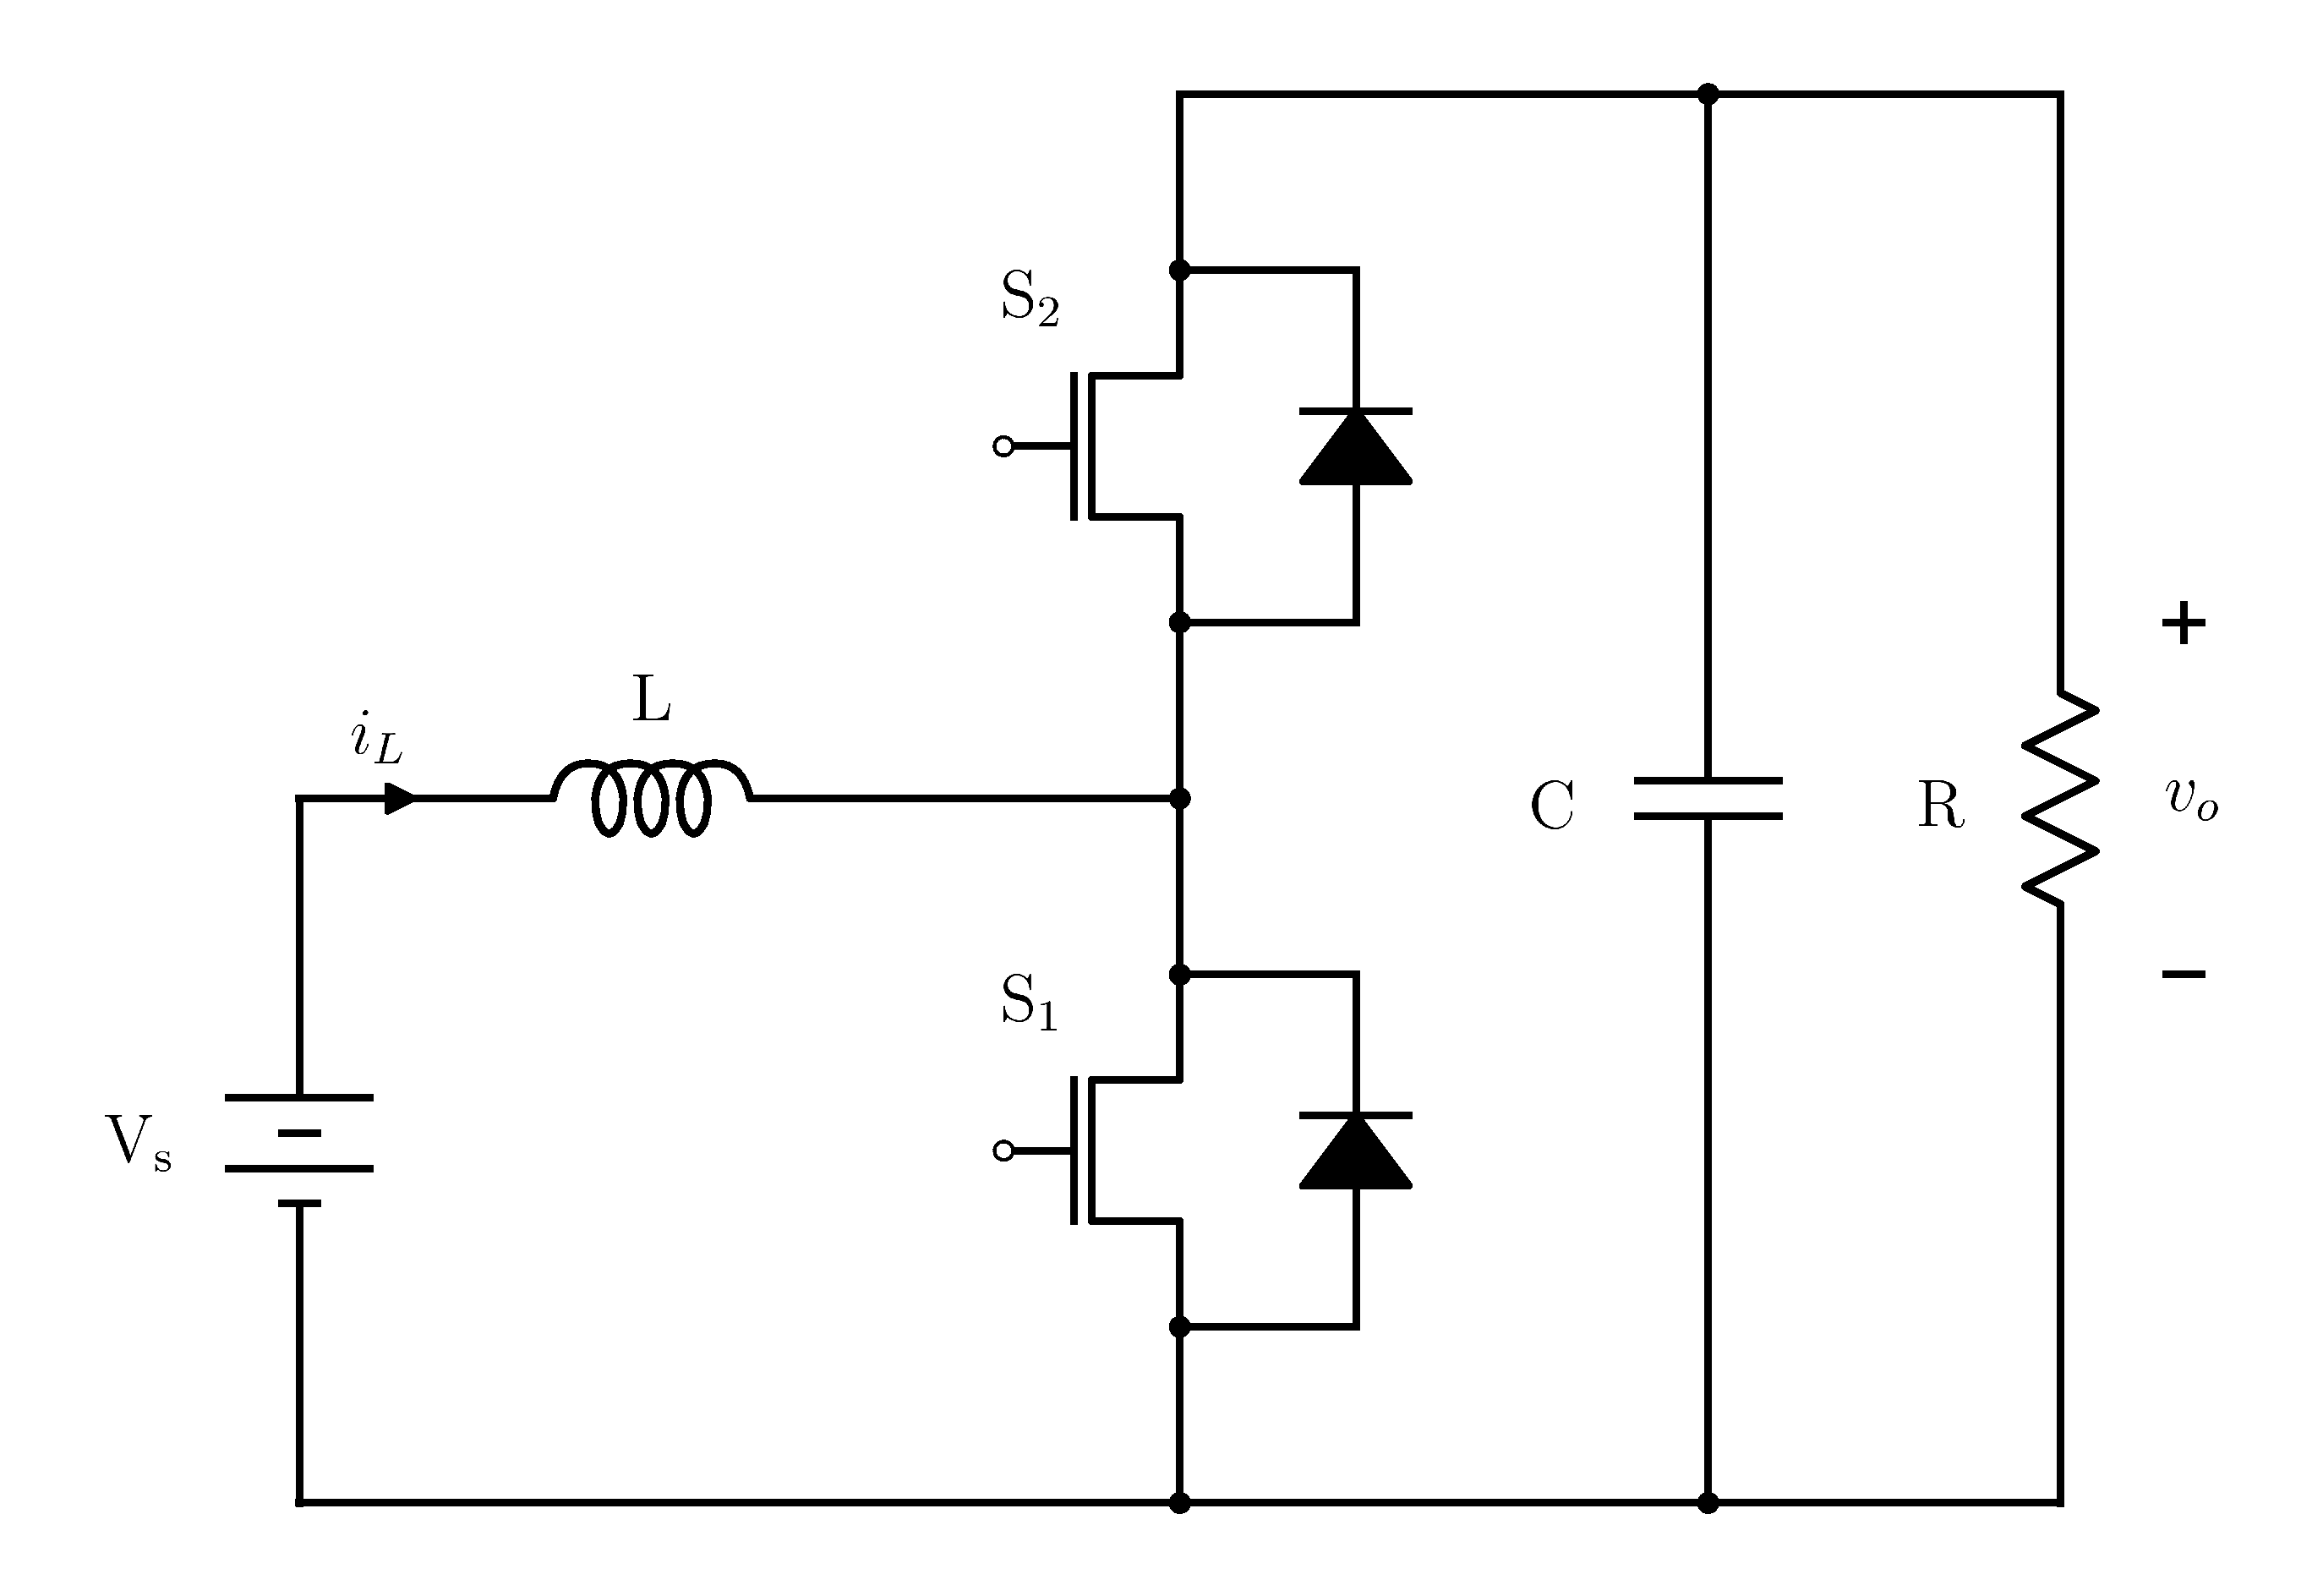
\includegraphics[width=0.46\columnwidth]{Imágenes/Diseño del control/Convertidor bidireccional de corriente.pdf}
  \caption{Convertidor elevador bidireccional en corriente.}
  \label{convertidor-bidireccional-diseno}
\end{figure} 

Las llaves $\mathrm{S_1}$ y $\mathrm{S_2}$ trabajan en forma complementaria: cuando $\mathrm{S_1}$ conduce, $\mathrm{S_2}$ no conduce, y viceversa. Con este pretexto y asumiendo que el convertidor se encuentra trabajando en modo de conducción continua (MCC), el mismo puede encontrarse en uno de los siguientes estados:

\begin{itemize}
    \item \textbf{$\boldsymbol{\mathrm{S_1}}$ conduce y $\boldsymbol{\mathrm{S_2}}$ no conduce}
    
    En este estado se analizan las ecuaciones de Kirchhoff para el circuito cerrado de la malla de la fuente y para las corrientes en el nodo de la carga. Expresándolas en función de la tensión en el inductor y la corriente por el capacitor, se obtienen las siguientes ecuaciones:

    \begin{equation}
        \begin{split}
          & L \frac{di_L(t)}{dt} = v_s(t) 
          \\
          & C \frac{dv_o(t)}{dt} = - \frac{v_o(t)}{R}
        \end{split}
        \label{sistema-modelo-1}
      \end{equation}

      \item \textbf{$\boldsymbol{\mathrm{S_1}}$ no conduce y $\boldsymbol{\mathrm{S_2}}$ conduce}
      
      Nuevamente expresando las ecuaciones de Kirchhoff correspondientes a este estado respecto la tensión en el inductor y la corriente en el capacitor se obtiene:
      
    \begin{equation}
        \begin{split}
          & L \frac{di_L(t)}{dt} = v_s(t) - v_o(t)
          \\
          & C \frac{dv_o(t)}{dt} = i_L(t)- \frac{v_o(t)}{R}
        \end{split}
        \label{sistema-modelo-2}
      \end{equation}
\end{itemize}

\subsection{Parametrizado mediante ciclo de trabajo}

Para unificar las Ecuaciones \ref{sistema-modelo-1} y \ref{sistema-modelo-2} hallados para el convertidor elevador en un solo sistema, se define la acción de control $u(t)$ de la siguiente forma:

\[
  u(t) = \left\{\begin{alignedat}{2}
    & 1 &\quad  \text{$S_1$ conduce y $S_2$ no conduce} \\
    & 0 &\quad  \text{$S_1$ no conduce y $S_2$ conduce} \\
  \end{alignedat}\right.
\]

Implementando esta condición para unir los sistemas de ecuaciones mencionados anteriormente se obtiene:

\begin{equation}
  \boxed{
    \begin{split}
      & L \frac{di_L(t)}{dt} = v_s(t) - \left[1-u(t)\right]v_o(t) \vspace{0.5cm}
      \\
      & C \frac{dv_o(t)}{dt} = \left[1-u(t)\right] i_L(t)- \frac{v_o(t)}{R}
  \end{split}
    }
  \label{sistema-modelo-param}
  \end{equation}

Este sistema de ecuaciones parametrizado es el típicamente usado para representar a los convertidores elevadores en la bibliografía de la temática.

\subsection{Promediado del sistema de ecuaciones}

En esta etapa se realiza una aproximación para poder simplificar las ecuaciones que definen el comportamiento de los mismos y así facilitar el tratamiento de los modelos resultantes.

Las Ecuaciones \ref{sistema-modelo-param} describen un \emph{sistema de estructura variable no lineal}, esto significa que el convertidor elevador se comporta como diferentes sistemas no lineales continuos en diferentes regiones de su estado de espacios, y este comportamiento se encuentra dictado por una acción de control $u(t)$ discontinua. Esto presenta una complejidad elevada en el análisis y control del sistema.

Una aproximación factible es el uso de \emph{medias móviles}, en las que cada señal se sustituye por su promedio durante un período de conmutación $T$. Este método permite modelar al sistema como uno de estructura no variable, debido a que la señal de control es continua bajo esta aproximación. Otra ventaja de las medias móviles es que al aplicarlo se obtiene la parte dominante de las señales y elimina las pequeñas perturbaciones, como el \emph{ripple} de conmutación, el cual no es de interés al diseñar el sistema de control para el conmutador.

Utilizando el método de promediado presentado en \cite{erickson} y \cite{hart} para simplificar las ecuaciones que rigen la dinámica del sistema:

\begin{equation}
  \left\langle x(t) \right\rangle_T = \frac{1}{T} \int_t^{t+T} x(\tau) \, d\tau
  \label{promediado}
\end{equation}

Puede demostrarse que aplicando la Ecuación \ref{promediado} a las Ecuaciones \ref{sistema-modelo-param} se obtiene:

\begin{equation}
  \boxed{
  \begin{split}
    & L \frac{d\left\langle i_L(t) \right\rangle_T}{dt} = \left\langle v_s(t) \right\rangle - \left[1-d(t)\right] \left\langle v_o(t) \right\rangle_T 
    \\
    & C \frac{d \left\langle v_o(t) \right\rangle_T}{dt} = \left[1-d(t)\right] \left\langle i_L(t) \right\rangle_T - \frac{\left\langle v_o(t) \right\rangle_T}{R}
  \end{split}
  }
  \label{sistema-modelo-prom}
\end{equation}

Siendo $d(t) = \left\langle u(t) \right\rangle_T$.

Cabe aclarar que es posible hallar un modelo promediado del convertidor trabajando en modo de conducción discontinua (MCD) \cite{jiansun}. Tal desarrollo no es presentado en este informe ya que escapa a los objetivos del presente trabajo.

\subsection{Linealización del sistema de ecuaciones}

Aún habiendo promediado al sistema, el modelo obtenido no es lineal, como se observa en las Ecuaciones \ref{sistema-modelo-prom} en las que aparecen productos entre los estados del sistema y la señal de control promediada $d(t)$. Como las técnicas tradicionales de análisis de sistemas (transformada de Laplace, diagramas de Bode, lugar de raíces, etc.) no son aplicables para el estudio de un modelo no lineal, es necesario linealizarlo.

Primero, ha de suponerse que el sistema ha sido llevado a un punto de trabajo fijo, en el que se encuentra con valores estacionarios en sus variables, a los que se hará referencia de la siguiente forma:

\begin{itemize}
  \item $I_{L_{ee}}$ es la \emph{corriente en la inductancia en estado estacionario}.
  \item $V_{o_{ee}}$ es la \emph{tensión en la salida en estado estacionario}.
  \item $V_{s_{ee}}$ es la \emph{tensión en la entrada en estado estacionario}.
  \item $D_{ee}$ es el \emph{ciclo de trabajo en estado estacionario}.
\end{itemize}

Al asumir que el sistema se encuentra en estado estacionario, las Ecuaciones \ref{sistema-modelo-prom} que definen la dinámica promedio del sistema se transforman en:

\begin{equation}
  \begin{split}
    & 0 = V_s - \left[ 1-D_{ee} \right] V_{o_{ee}}
    \\
    & 0 = \left[ 1-D_{ee} \right] I_{L_{ee}} - \frac{V_{o_{ee}}}{R}
  \end{split}
  \label{sistema-modelo-ee}
\end{equation}

Puede observarse que el comportamiento en este punto de trabajo coincide con el análisis efectuado en el capítulo de conversor elevador para modo de conducción continua, obteniéndose la misma relación de conversión (Ec. \ref{salida-elevador}).

Conocido el comportamiento del sistema en régimen de estado estacionario, se procede a la linealización del modelo. Este procedimiento consiste en realizar una aproximación de primer orden de las ecuaciones no lineales que describen al sistema, en un entorno muy cercano al punto de trabajo.

Para esto, primero debe construirse un \emph{modelo de pequeña señal} alrededor del punto de trabajo. Si se asume que el ciclo de trabajo promedio $d(t)$ es igual a un valor de estado estacionario $D$ más una perturbación denotada por $\hat{d}(t)$ se obtiene:

\begin{equation}
  \left\langle u(t) \right\rangle_T = d(t) = D_{ee} + \hat{d}(t)
  \label{ciclo-lineal} 
\end{equation}

Se asume que el valor de la perturbación $\hat{d}(t)$ es mucho menor que el valor de estado estacionario $D$, de modo que el valor promedio del ciclo de trabajo se mantendrá siempre cercano a este último. La respuesta del sistema ante esta perturbación de entrada resulta en los valores promedios de las variables:

\begin{equation}
  \begin{split}
    & \left\langle v_o(t) \right\rangle_T = V_{o_{ee}} + \hat{v_o}(t)
    \\
    & \left\langle i_L(t) \right\rangle_T = I_{L_{ee}} + \hat{i_L}(t)
  \end{split}
  \label{sistema-modelo-prom-ee}
\end{equation}

Las perturbaciones presentes en las Ecuaciones \ref{sistema-modelo-prom-ee} se consideran muy pequeñas con respecto a los valores de estado estacionario. Substituyendo los valores promedio definidos por las Ecuaciones~\ref{ciclo-lineal}~y~\ref{sistema-modelo-prom-ee} en el sistema promediado dado por las Ecuaciones \ref{sistema-modelo-prom}:

\begin{equation}
  \begin{split}
    & L \frac{d \left[ I_{L_{ee}} + \hat{i_L}(t)\right]}{dt} = V_s - \left[ 1 - D_{ee} - \hat{d}(t) \right] \, \left[ V_{o_{ee}} + \hat{v_o}(t) \right]
    \\
    & C \frac{d \left[ V_{o_{ee}} + \hat{v_o}(t)\right]}{dt} = V_s - \left[ 1 - D_{ee} - \hat{d}(t) \right] \, \left[ I_{L_{ee}} + \hat{i_L}(t) \right] - \left[ \frac{V_{o_{ee}}}{R} + \frac{\hat{v_o}(t)}{R} \right]
  \end{split}
\end{equation}

Operando:

\begin{equation}
  \begin{split}
    & L \frac{d \hat{i_L}(t)}{dt} = V_s -  (1 - D_{ee}) \, V_{o_{ee}} - (1 - D_{ee}) \, \hat{v_o}(t) + \hat{d}(t) V_{o_{ee}} + \hat{d}(t) \hat{v_o}(t)
    \\
    & C \frac{d \hat{v_o}(t)}{dt} = (1 - D_{ee}) \, I_{L_{ee}} + (1 - D_{ee}) \, \hat{i_L}(t) - \hat{d}(t) \, I_{L_{ee}} - \hat{d}(t) \, \hat{i_L}(t) - \frac{V_{o_{ee}}}{R} - \frac{\hat{v_o}(t)}{R}
  \end{split}
\end{equation}
Estas ecuaciones se simplifican considerando que:

\begin{itemize}
  \item $V_s = (1-D_{ee}) \, V_{o_{ee}}$
  \item $\frac{V_{o_{ee}}}{R} = I_{o_{ee}} = (1-D_{ee}) \, I_{L_{ee}}$
  \item Se eliminan los términos no lineales de segundo orden que se presentan al considerarse que las perturbaciones son muy pequeñas, y el producto entre ellas lo son aún más.
\end{itemize}

El resultado es el modelo lineal del convertidor:

\begin{equation}
  \boxed{
  \begin{split}
  & L \frac{d\hat{i_L}(t)}{dt} = - (1-D_{ee}) \, \hat{v_o}(t) + \hat{d}(t) \, V_{o_{ee}}
  \\ 
  & C \frac{d\hat{v_o}(t)}{dt} = - (1-D_{ee}) \, \hat{i_L}(t) - \hat{d}(t) \, I_{L_{ee}} - \frac{\hat{v_o}(t)}{R}  
  \end{split}
  }
  \label{sistema-modelo-lineal}
\end{equation}

\section{Diseño del sistema de control}

El primer paso en el diseño del sistema de control consiste en definir qué tipo de señal se utilizará como excitación en el gate de los transistores del convertidor. Dos alternativas son presentadas:

\begin{itemize}
  \item Los \textbf{sistemas de control a frecuencia fija} poseen un ciclo de trabajo variable, pero la frecuencia es constante. Un ejemplo es la modulación por ancho de pulso o PWM (del inglés \emph{pulse width modulation}).
  \item Los \textbf{sistemas de control a frecuencia variable} mantienen constante el tiempo durante el cual el transistor es excitado con un nivel alto, pero la frecuencia de su conmutación es variable. Un ejemplo es la modulación de la frecuencia del pulso o PFM (del ingles \emph{pulse frequency modulation}).
\end{itemize}

El control por PWM presenta una menor eficiencia que el control por PFM con cargas pequeñas, debido a que este último reduce la frecuencia de su señal en estos casos, lo que conlleva menores pérdidas por conmutación de las llaves. Aun así, el control por PWM es preferible debido a su frecuencia fija, lo que significa que el \emph{ripple} de conmutación se encuentra acotado, y simplifica de gran manera la implementación de la acción de control, mientras que en el control por PFM el rizado puede tener amplitudes mayores cuando se reduce mucho la frecuencia. Por esta razón se utiliza este un control con señal de modulación de ancho de pulso para este trabajo.

El siguiente paso es comenzar a diseñar la estrategia de control, la cual se verá afectada por las especificaciones disponibles en cuanto a modos de funcionamiento y las características de la respuesta dinámica requerida. Específicamente para este trabajo, el objetivo de la acción de control es mantener una tensión constante en la carga.

Proponiendo un lazo de realimentación como el de la Figura \ref{lazo-tension-propuesto}, se observa rápidamente que esta estrategia no es viable cuando la planta es un convertidor elevador.

\begin{figure}[hbt!]
  \centering
  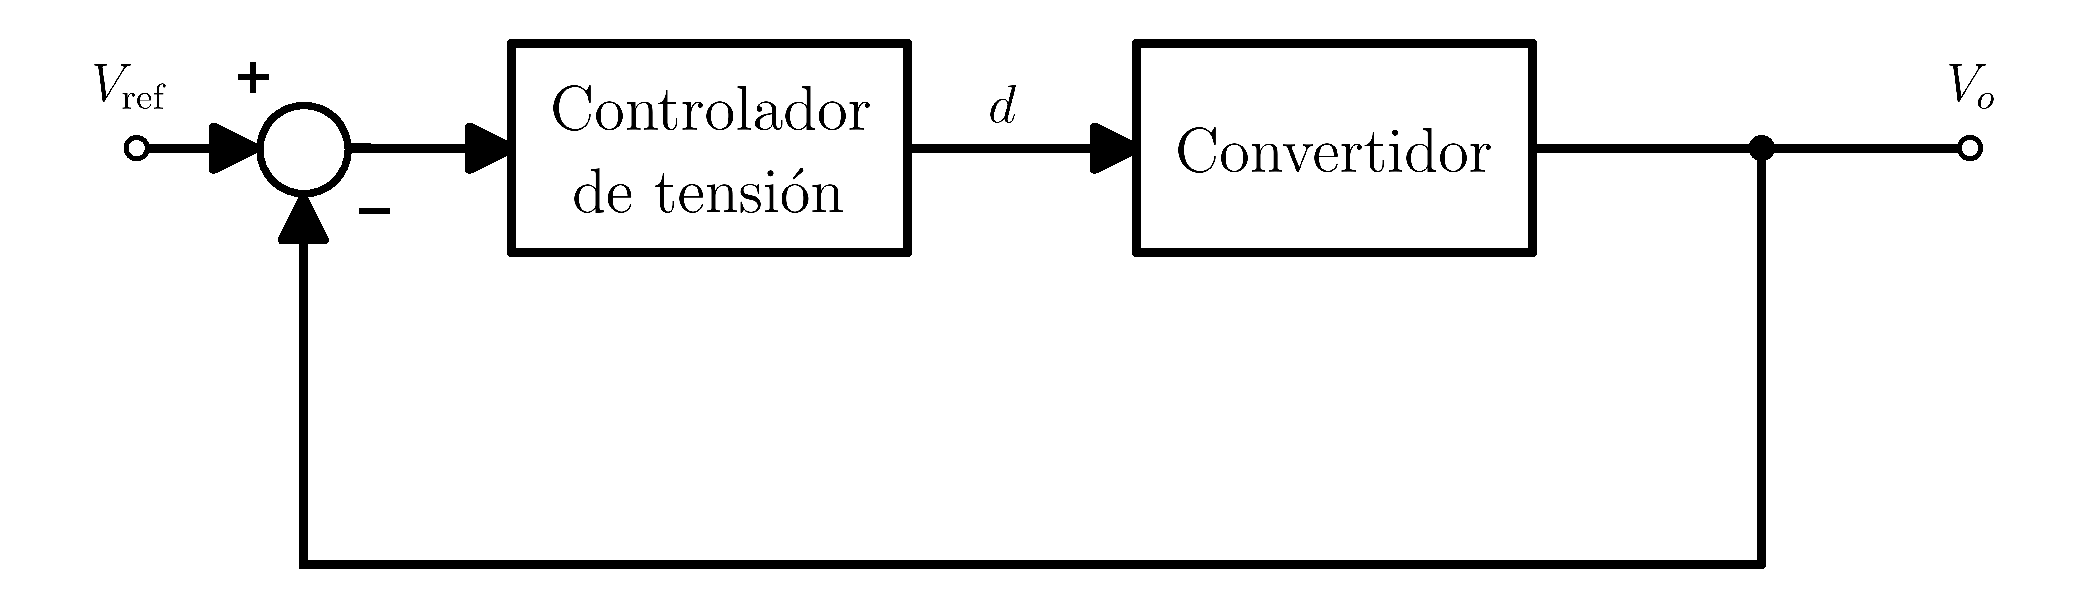
\includegraphics[width=0.65\columnwidth]{Imágenes/Diseño del control/Primer lazo de control de tensión.pdf}
  \caption{Ilustración del lazo de control de tensión propuesto.}
  \label{lazo-tension-propuesto}
\end{figure} 

Esta impracticabilidad se demuestra asumiendo inicialmente que la tensión de salida se ha estabilizado en un valor estacionario $V_{o_{ee}}$ y considerando una tensión de entrada constante $V_s$. Substituyendo estos valores en las Ecuaciones \ref{sistema-modelo-prom} correspondientes al sistema promediado:

\begin{equation*}
  \begin{split}
    & L \frac{d\left\langle i_L(t) \right\rangle_T}{dt} = V_s - \left[1-d(t)\right] \, V_{o_{ee}}
    \\
    & 0 = \left[1-d(t)\right] \left\langle i_L(t) \right\rangle_T - \frac{V{o_{ee}}}{R}
  \end{split}
\end{equation*}

Realizando un reemplazo sobre el ciclo de trabajo promediado se obtiene:

\begin{equation}
  L \frac{d\left\langle i_L(t) \right\rangle_T}{dt} = V_s - \frac{V_{o_{ee}^2}}{R \, \left\langle i_L(t) \right\rangle_T}
  \label{prueba-inestabilidad-lazo}
\end{equation}

Y efectuando otro reemplazo con la potencia de salida $P_{o_{ee}} = V_{o_{ee}}^2/R$ se obtiene:

\begin{equation*}
  L \frac{d\left\langle i_L(t) \right\rangle_T}{dt} = V_s - \frac{P_{o_{ee}}}{\left\langle i_L(t) \right\rangle_T}
\end{equation*}

Dado que la potencia de salida es siempre menor a la de la entrada debido a pérdidas, se tiene:

\begin{equation*}
  \frac{P{o_{ee}}}{\left\langle i_L(t) \right\rangle_T} < \frac{P{s_{ee}}}{\left\langle i_L(t) \right\rangle_T}
\end{equation*}

\begin{equation*}
  \boxed{\frac{P{o_{ee}}}{\left\langle i_L(t) \right\rangle_T} < V_s \quad \forall \quad t}
\end{equation*}

Esto implica que el miembro derecho de la Ecuación \ref{prueba-inestabilidad-lazo} es mayor que cero para todo instante de tiempo, por lo que la derivada de la corriente es siempre positiva, y en consecuencia la corriente por el inductor diverge. 

La razón por la que esto ocurre es que hay una parte de la dinámica del sistema que no está siendo controlada. Es decir, si solamente se controla la tensión de salida, la corriente por el inductor se deja variar en forma libre. Esta dinámica de lazo cerrado para estados no controlados de un sistema no lineal se conoce como \emph{dinámica escondida} o \emph{dinámica cero}, y su estabilidad es condición necesaria para la estabilidad del sistema entero \cite{dynamics}. Dado que la dinámica cero del convertidor con un lazo cerrado de tensión resulta inestable, se concluye que es necesario implementar un control de corriente anidado dentro del lazo de tensión. En resumen, la estrategia de control consiste en:

\begin{enumerate}
  \item El \textbf{lazo interno de control de corriente}, el cual se encarga de la dinámica escondida de esta variable de estado.
  \item El \textbf{lazo externo de control de tensión}, el cual se encarga de generar la acción de control para cumplir el objetivo de mantener la tensión de carga constante. Este lazo es el encargado de calcular e inyectar la referencia en el lazo interno.
\end{enumerate}

Por eso mismo, se realizará un diseño en fases para cumplir individualmente estos objetivos, cuya primer etapa será el diseño del lazo interno de corriente.

\subsection{Diseño del lazo interno de corriente}

Dado el contexto de un sistema de control de tensión, para el diseño del lazo de corriente se asume una tensión constante, y se controla el flujo de la potencia en forma indirecta mediante el control de la componente media de la corriente por el inductor. 

La Figura \ref{lazo-corriente} representa el modo de control propuesto para la corriente del convertidor electrónico. Este consiste en un lazo de realimentación que permite comparar la corriente en el inductor con la referencia de corriente deseada, para inyectar con la señal error resultante a un controlador en cascada con el sistema.

\begin{figure}[hbt!]
  \centering
  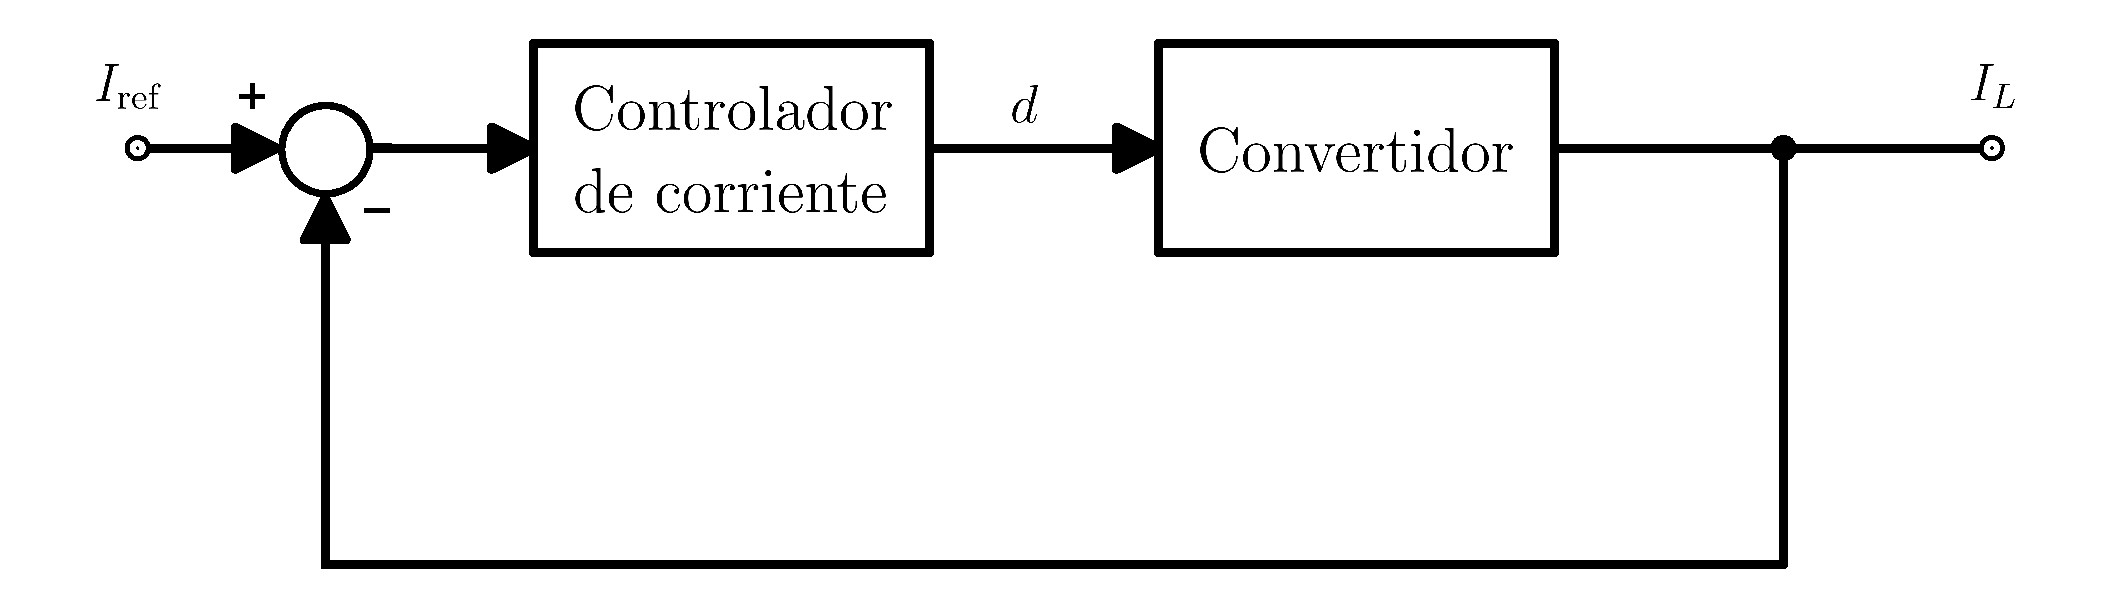
\includegraphics[width=0.65\columnwidth]{Imágenes/Diseño del control/Lazo de control de corriente.pdf}
  \caption{Ilustración del lazo de control de corriente.}
  \label{lazo-corriente}
\end{figure} 

El modelo linealizado del convertidor elevador obtenido en las Ecuaciones \ref{sistema-modelo-lineal} permite aplicar herramientas convencionales de análisis como la transformada de Laplace, lugar de raíces, entre otros. Por su parte, como se aclaró en el Capítulo \ref{cap-fpga}, el hardware de control será un FPGA, el cual opera a partir de muestras obtenidas mediante dos conversores. Por esto mismo, el diseño del controlador se realiza en el dominio discreto.

El primero paso a realizar es obtener la función de transferencia continua del convertidor, aplicando la transformada de Laplace a las Ecuaciones \ref{sistema-modelo-lineal}, y asumiendo que las condiciones iniciales son nulas. Las siguientes ecuaciones son obtenidas

\begin{equation}
  \begin{split}
    & s \, L \, I_L(s) = - \left( 1 - D_{ee} \right) \, V_o(s) + V_{o_{ee}} \, D(s)
    \\
    & s \, C \, V_o(s) = - \left( 1 - D_{ee} \right) \, I_L(s) + I_{L_{ee}} \, D(s) - \frac{V_o(s)}{R}
    \label{sistema-modelo-laplace}
  \end{split}
\end{equation}

Considerando como salida a la corriente del inductor $I_L$ y como entrada al ciclo de trabajo $D$, se obtiene la función de transferencia expresada en la Ecuación \ref{transferencia-corriente-inductor}.

\begin{equation}
  \boxed{G_{I_L}(s) = \frac{I_L(s)}{D(s)} = \frac{\frac{V_{o_{ee}}}{L} \, s + \left[ \frac{I_{L_{ee} \, (1 - D_{ee})}}{L \, C} + \frac{V_{o_{ee}}}{L\,C\,R} \right]}{s^2 + \frac{1}{R\,C} \, s + \frac{\left( 1 - D_{ee} \right)^2}{L \, C}}}
  \label{transferencia-corriente-inductor}
\end{equation}

Ahora, deben seleccionarse valores de tensión de entrada $V_s$, ciclo de trabajo $D_{ee}$, y resistencia de carga $R$ que conforman el punto de operación alrededor del cual se trabajará con el sistema. Considerando una tensión un poco menor de la nominal del banco de supercapacitores y baterías de litio, se obtiene la asignación mostrada en la Tabla \ref{punto-trabajo-convertidor}.

\begin{table}[hbt!]
  \centering
  \begin{tabular}{l|l}
  $V_s$     & \SI{25}{\volt} \\
  $D_{ee}$    & 0.5 \\
  $R$        & \SI{15}{\ohm}  \\
  $V_{o_{ee}}$ & \SI{50}{\volt} 
  \end{tabular}
  \caption{Punto de trabajo alrededor del cual se linealiza el convertidor}
  \label{punto-trabajo-convertidor}
\end{table}

En el convertidor elevador utilizado, los valores de inductancia y capacitancia por diseño son de \SI{200}{\micro\henry} y \SI{200}{\micro\farad}, respectivamente. Con estos valores y reemplazando en la Ecuación \ref{transferencia-corriente-inductor}:

\begin{equation}
  \boxed{G_I(s) = \frac{I_L(s)}{D(s)} = \frac{250\,000\,s + 15.15 \times 10^6}{s^2 + 30.3 \, s + 568.18 \times 10^3}}
  \label{planta-valores}
\end{equation}

Cuyos polos complejos conjugados se encuentran en -15.15 $\pm$ $j$753.62. 

La discretización de la planta depende del tiempo de muestreo $T_s$ de los conversores analógico-digitales, el cual debe ser varias veces menor que la menor constante de tiempo del sistema. Para esto, se programa al controlador de los ADCs para que tengan un período de muestreo de \SI{1.6}{\micro\second}, bien por debajo del período de conmutación de las llaves de \SI{50}{\micro\second}. La aproximación utilizada para la discretización de la planta es el método de \emph{Euler en avance}:

\begin{equation}
  s = \frac{z-1}{T_s}
  \label{euler-avance}
\end{equation}

En donde $T_s$ es el período de muestreo anteriormente mencionado. Reemplazando la Ecuación \ref{euler-avance} en la Ecuación \ref{planta-valores}:

\begin{equation}
  \boxed{G_I(z) = \frac{0.4(z-0.999903)}{z^2 - 1.99995z  + 0.999953}}
  \label{modelo-discretizado}
\end{equation}

Una vez obtenido el modelo discretizado, es necesario seleccionar el tipo de controlador a implementar. Las especificaciones buscadas en cuanto la respuesta dinámica de la corriente en el inductor son:

\begin{itemize}
  \item Error de estado estacionario nulo.
  \item Tiempo de establecimiento del orden del milisegundo o menor.
  \item Si se producen sobrepicos, que su amplitud no ponga en riesgo a los componentes del sistema, ni a la carga.
\end{itemize}

Se optó por la implementación de un control tipo proporcional-integral-derivativo digital, más comúnmente llamados por su acrónimo \emph{controlador PID}.

\subsubsection{Controladores PID}
\label{diseno-controladores-pid}

Los controladores PID (Figura \ref{esquema-pid}) son controladores que tienen una larga historia en el campo de control automático. Debido a su mecanismo intuitivo y su relativa simpleza, además de una performance satisfactoria en un amplio rango de procesos, se consideran el controlador estándar en la industria. Aplicar una ley de control PID consiste en aplicar la suma de tres tipos de acciones de control: una acción proporcional, una integral, y una derivativa.

\begin{figure}[hbt!]
  \centering
  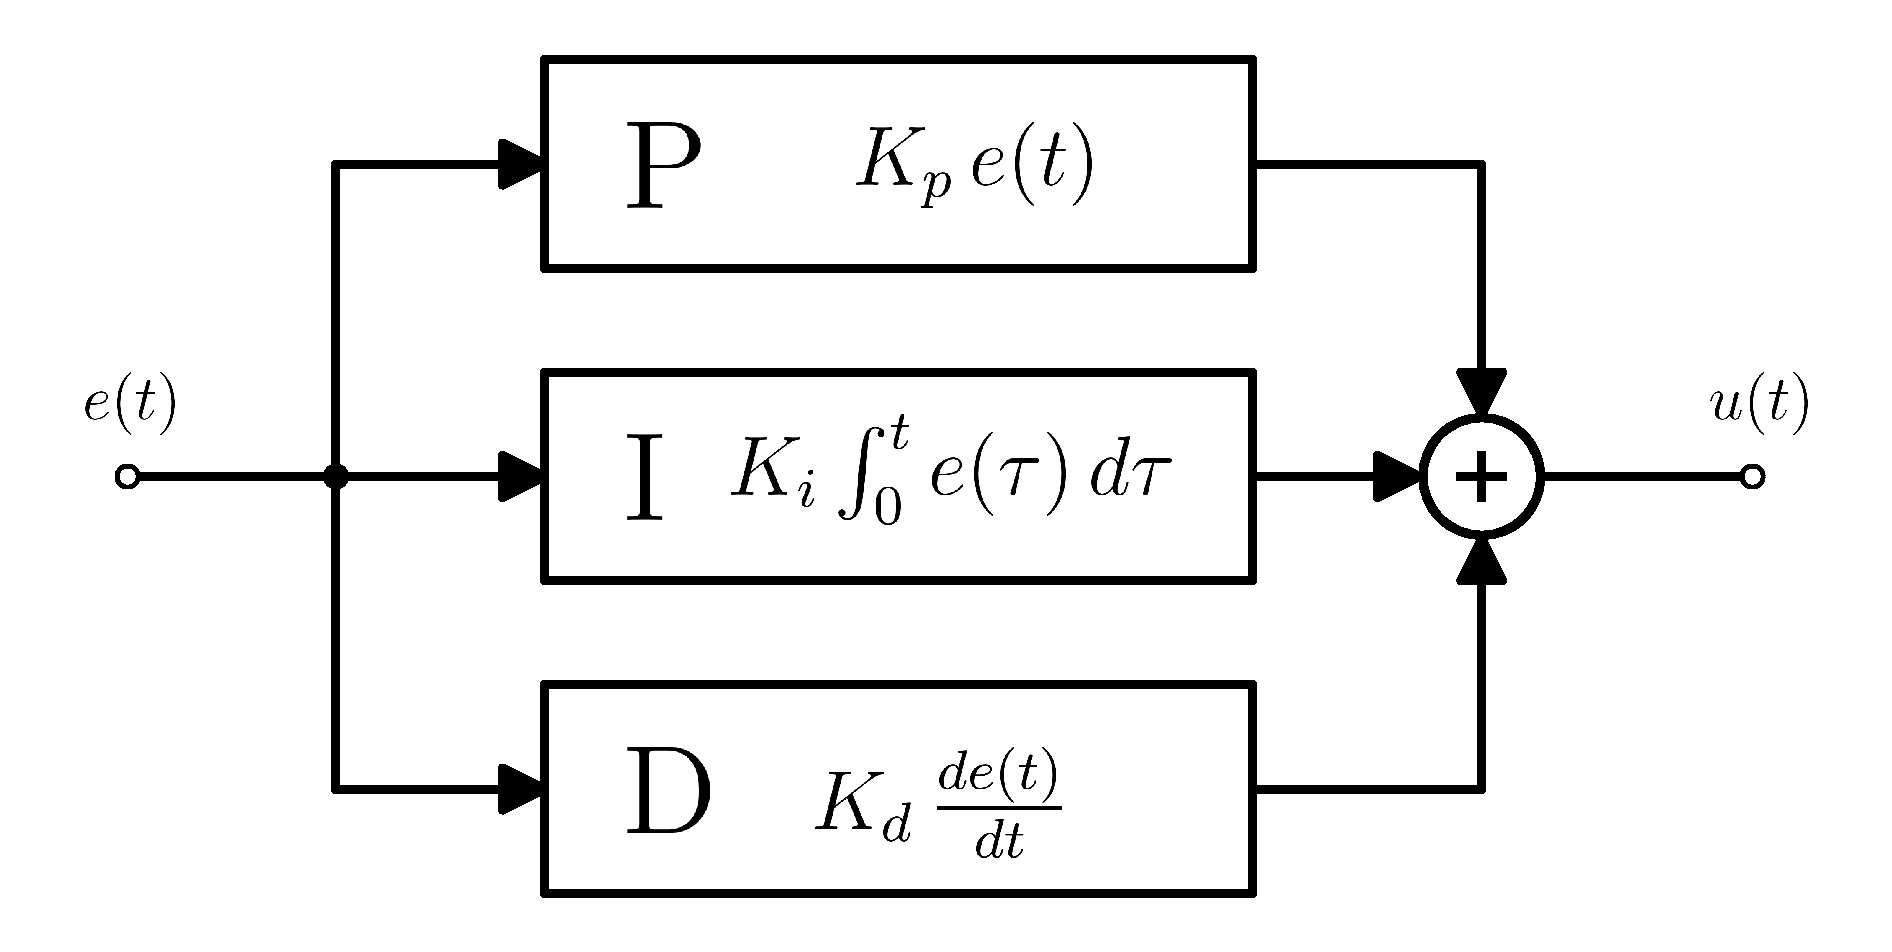
\includegraphics[width=0.45\columnwidth]{Imágenes/Diseño del control/Controlador PID.pdf}
  \caption{Diagrama en bloques de un controlador PID.}
  \label{esquema-pid}
\end{figure} 

\begin{itemize}
  \item La \textbf{acción proporcional} es proporcional a la señal error que ingresa al controlador, dada por la expresión
  \begin{equation*}
    u(t) = K_p \, e(t) = K_p \left( r(t) - y(t) \right)
  \end{equation*}
  en donde $K_p$ es la ganancia proporcional. Su significado es sencillo, ya que su comportamiento es aumentar la variable de control cuando el error es grande, con su signo apropiado. La mayor desventaja de usar un controlador proporcional puro es que produce un error de estado estacionario, aún cuando la planta presente una dinámica integral (es decir, su función de transferencia presenta un polo en el origen del plano complejo).
  \item La \textbf{acción integral} es proporcional a la integral del error del control, es decir
  \begin{equation*}
    u(t) = K_i \, \int_{0}^{t} e(\tau) \, d\tau
  \end{equation*}
  en donde $K_i$ es la ganancia integral, y su función de transferencia es:
  \begin{equation*}
    C(s) = \frac{K_i}{s}
  \end{equation*}

  La presencia del polo en el origen permite la reducción a cero del error de estado estacionario cuando una señal escalón es aplicada en la referencia o cuando ocurre una perturbación en la carga. Aún así, cuando se presenta una acción integral, el llamado efecto \emph{windup} puede ocurrir en el caso de que se presente una saturación en la variable de control.

  Esta situación se da debido a que el integrador del controlador no conoce los límites físicos del sistema a controlar y por lo tanto, ante ciertas situaciones (por ejemplo, un gran cambio en la referencia), es posible que la acción de control generada exceda estas limitaciones, lo que puede causar un sobrepico en alguna variable de estado del sistema. Para evitar este problema se utilizan métodos \emph{anti-windup}.
  \item Mientras la acción proporcional se basa en el valor presente del error de control y la acción integral se basa en sus valores pasados, la \textbf{acción derivativa} se basa en predecir futuros valores de esta señal. Una ley de control derivativa ideal puede ser expresada como:
  \begin{equation*}
    u(t) = K_d \, \frac{d e(t)}{dt}
  \end{equation*}
  en donde $K_d$ es la ganancia derivativa, y su función de transferencia es 
  \begin{equation*}
    C(s) = K_d \, s 
  \end{equation*}
  Este tipo de acción de control tiene un gran potencial en mejorar la performance del control, debido a que podría anticipar una incorrecta tendencia en la señal error y contrarrestarla. Sin embargo, también posee algunas cuestiones críticas que hacen que no sea adoptada en casos prácticos. Específicamente en el marco de este trabajo y debido a la conmutación de las llaves y la generación del ripple presente en las variables de estado a controlar, el término derivativo termina amplificando este rizado, lo cual es indeseado y podría generar una oscilación en el sistema de control. Por esto mismo, se decide implementar un controlador proporcional-integral (PI).
\end{itemize}

La transferencia discreta de un PI suele expresarse como: 

\begin{equation*}
  \mathrm{PI}_I(z) = K_p + \frac{K_i \, T_s}{z-1}
\end{equation*}

Y las ganancias proporcional e integral $K_p$ y $K_i$ deben ser balanceadas a partir de la sintonización del controlador PI para obtener la performance buscada a lazo cerrado. En la Sección \ref{implementacion-pid} del Capítulo \ref{implementacion-control} se detalla la implementación del método de \emph{anti-windup} para la acción de control integral, conocido como \emph{clamping}. El clamping consiste en deshabilitar el integrador cuando una cierta condición es alcanzada. Las siguientes opciones pueden ser implementadas:

\begin{itemize}
  \item El término integral se limita a un valor predefinido.
  \item La integración se detiene cuando el error es mayor a un umbral predefinido, es decir, cuando la variable de estado del proceso está muy lejos de la referencia.
  \item La integración se detiene caundo la variable de control se satura, es decir, cuando $u \neq u'$.
  \item La integración se detiene cuando la variable de control se satura, y tiene la misma señal que la señal error, es decir, cuando $u \cdot e > 0$.
\end{itemize}

El método utilizado en este trabajo es el primero, en el cual se realiza una saturación del término integral.

\subsubsection{Filtro de corriente}
\label{diseno-filtro-corriente}

Como se mencionó anteriormente, la acción de control será calculada a partir de la corriente media por el inductor, y no su valor instantáneo. Por esto mismo resulta necesario aplicar a la señal de corriente medida un filtro pasa-bajo que rechace las componentes del \emph{ripple}, y que además sea lo suficientemente rápido para poder seguir la dinámica de la planta modelada en la Ecuación \ref{planta-valores}. Dado que este rizado es producto de la conmutación de las llaves y su frecuencia fundamental es de \SI{20}{\kilo\hertz}, y los polos de la planta poseen un valor absoluto aproximado de 750, se decide implementar un filtro pasabajos de primer orden con frecuencia de corte en \SI{1.5}{\kilo\hertz}. La Figura \ref{filtro-corriente} muestra la forma en la que se incorpora este filtro al lazo interno de realimentación de corriente.

\begin{figure}[hbt!]
  \centering
  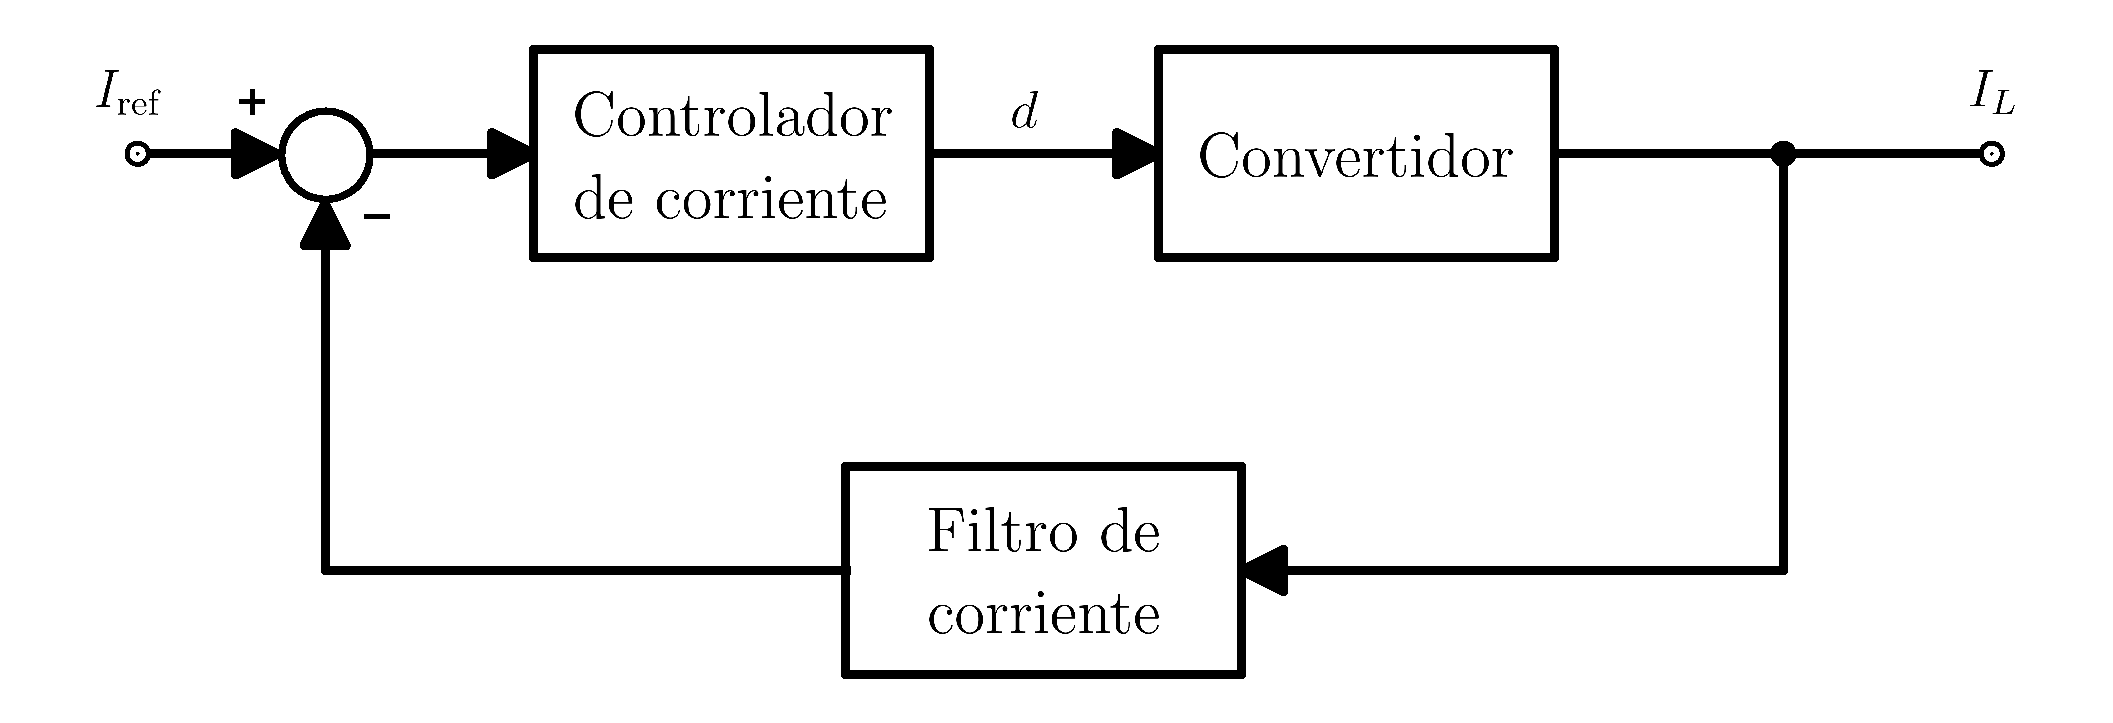
\includegraphics[width=0.65\columnwidth]{Imágenes/Diseño del control/Lazo de control de corriente con filtro.pdf}
  \caption{Lazo de control de corriente con filtro pasa-bajo.}
  \label{filtro-corriente}
\end{figure} 

Para esto, se partió de la transferencia en continua del filtro de primer orden a implementar:

\begin{equation}
  F_I(s) = \frac{\omega_c}{s+\omega_c} = \frac{2\pi \, 1.5 \times 10^3 }{s+ 2\pi \, 1.5 \times 10^3}
\end{equation}

Y luego se transformó al dominio discreto, nuevamente mediante el método de Euler en avance y la frecuencia de muestreo establecida anteriormente:

\begin{equation}
  \boxed{F_I(z) = \frac{0.0150796}{z-0.98492}}
  \label{filtro-corriente-discretizado}
\end{equation}

\subsubsection{Simulación del lazo interno de corriente}

Luego de filtrar correctamente la corriente por el inductor del convertidor, se procede al ajuste de los parámetros del controlador proporcional-integral. Para ello, la sintonización inicial fue hecha a partir de la transferencia lineal encontrada en la Ecuación \ref{modelo-discretizado} y las herramientas de simulación y cálculo provistas por MATLAB\textsuperscript\textregistered \hspace{0.6pt} y Simulink\textsuperscript\textregistered.

En la Figura \ref{simulacion-modelo-discretizado-corriente} puede observarse el esquema realizado para una primer simulación respecto de la transferencia discretizada del modelo. Para este paso fue utilizada la herramienta de sintonización provista por Simulink\textsuperscript\textregistered, la cual cuenta con dos controles deslizantes (Figura \ref{tuner-modelo-discretizado-corriente}) los cuales permiten ajustar la rapidez de la respuesta temporal y el comportamiento transitorio de la acción de control, y en base a eso, generar los parámetros del controlador.

\begin{figure}[hbt!]
  \centering
  \includegraphics[width=0.55\columnwidth]{Imágenes/Diseño del control/Simulación del lazo de corriente/Primer simulación del lazo de corriente.pdf}
  \caption{Primer simulación del lazo de control de corriente.}
  \label{simulacion-modelo-discretizado-corriente}
\end{figure} 

\begin{figure}[hbt!]
  \centering
  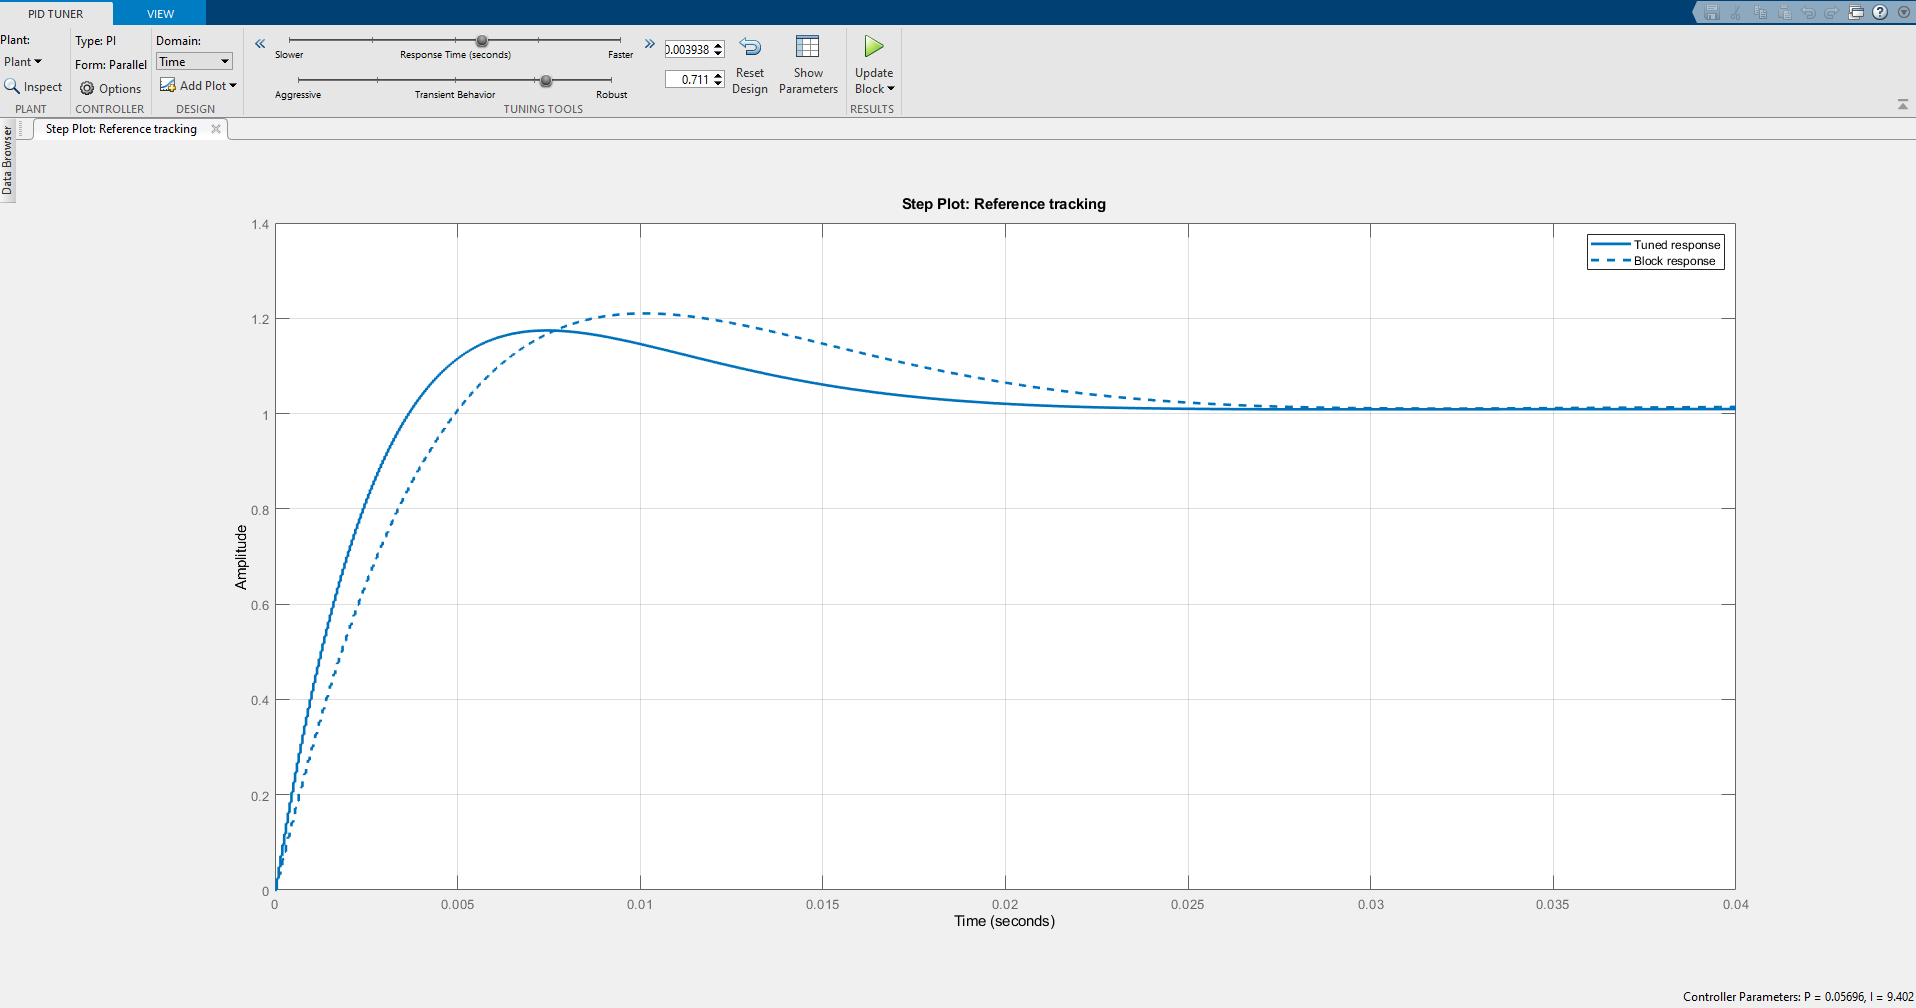
\includegraphics[width=0.70\columnwidth]{Imágenes/Diseño del control/Simulación del lazo de corriente/Tuner de Simulink.png}
  \caption{Sintonización del PI mediante herramientas de Simulink\textsuperscript\textregistered.}
  \label{tuner-modelo-discretizado-corriente}
\end{figure} 

Una vez generada una primer aproximación del lazo de control con una respuesta satisfactoria, se reemplaza al modelo linealizado del convertidor por el modelo real parametrizado, expresado por las Ecuaciones \ref{sistema-modelo-param}, y se implementa el filtro de corriente, como se observa en la Figura \ref{simulacion-modelo-real-corriente}. En esta simulación se inyecta un escalón unitario de \SI{8}{\ampere} a \SI{9}{\ampere} en la referencia del lazo de control de corriente y se observan las variables de estados del convertidor (corriente por el inductor y tensión en el capacitor o de salida), además de corroborar el funcionamiento del filtro implementado.

Analizando el comportamiento transitorio obtenido con la simulación del modelo real y realizando nuevos ajustes de manera de obtener una performance satisfactoria, se llega al siguiente controlador:

\begin{equation*}
  \boxed{\mathrm{PI}_I (z) = 0.02 + \frac{12 \cdot 1.6 \times 10^{-6}}{z-1}}
\end{equation*}

Donde se deduce que la constante proporcional $K_p$ es 0.02, y la constante integral $K_i$ es 12.

\begin{figure}[hbt!]
  \centering
  \includegraphics[width=0.72\columnwidth]{Imágenes/Diseño del control/Simulación del lazo de corriente/Simulación real del lazo de corriente.pdf}
  \caption{Simulación real del lazo de control de corriente.}
  \label{simulacion-modelo-real-corriente}
\end{figure} 

En la Figura \ref{formas-onda-lazo-corriente} se grafican los resultados de la simulación. A partir de la corriente por el inductor filtrada (Figura \ref{formas-onda-lazo-corriente}c), la cual atenúa satisfactoriamente al rizado de la forma de onda, se realiza un análisis del transitorio del escalón unitario aplicado. Utilizando las herramientas provistas por Simulink\textsuperscript\textregistered, se mide un valor de sobrepico del 1.8\% respecto del valor de estado estacionario de \SI{9}{\ampere}, y un tiempo de establecimiento con criterio del 2\%\footnote{Se entiende como \emph{tiempo de establecimiento del 2\%} al tiempo que tarda la señal en situarse en un entorno del 2\% alrededor del valor de estado estacionario.} de aproximadamente \SI{1}{\milli\second}.

En la Figura \ref{formas-onda-filtradas-lazo-corriente} se observa con mayor detalle la acción del filtro alrededor del punto de salto del escalón.

\begin{figure}[hbt!]
  \centering
  \subfloat[Referencia de corriente.]{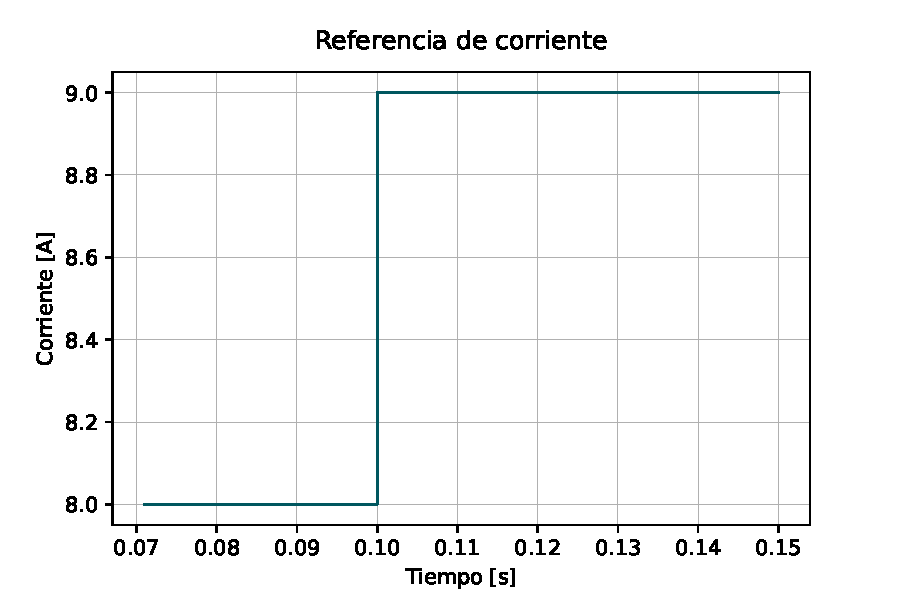
\includegraphics[width=0.45\textwidth]{Imágenes/Diseño del control/Simulación del lazo de corriente/Referencia de corriente.pdf}}    
  \hspace{3.5mm}
  \subfloat[Corriente por el inductor.]{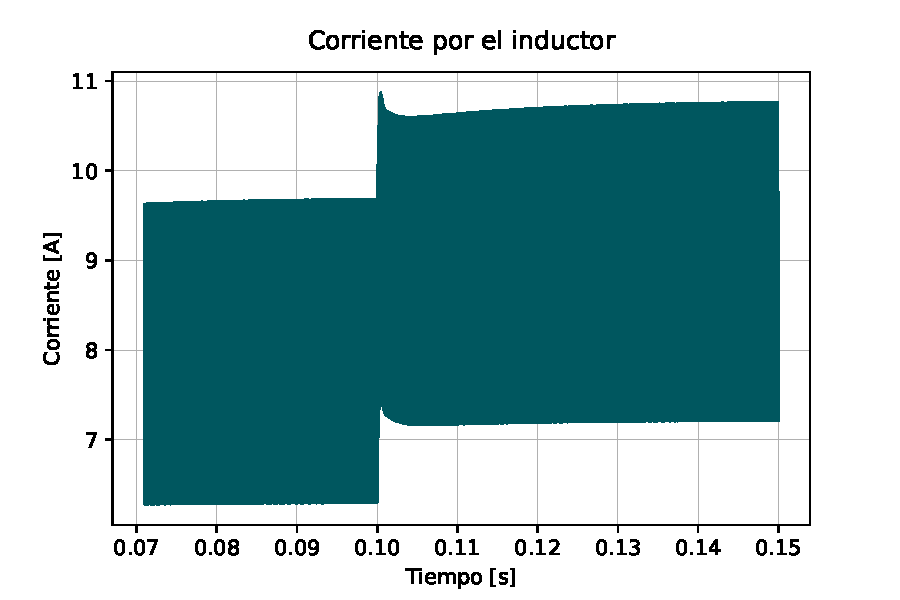
\includegraphics[width=0.45\textwidth]{Imágenes/Diseño del control/Simulación del lazo de corriente/Corriente por el inductor.pdf}}
  \hspace{3.5mm}
  \subfloat[Corriente por el inductor filtrada.]{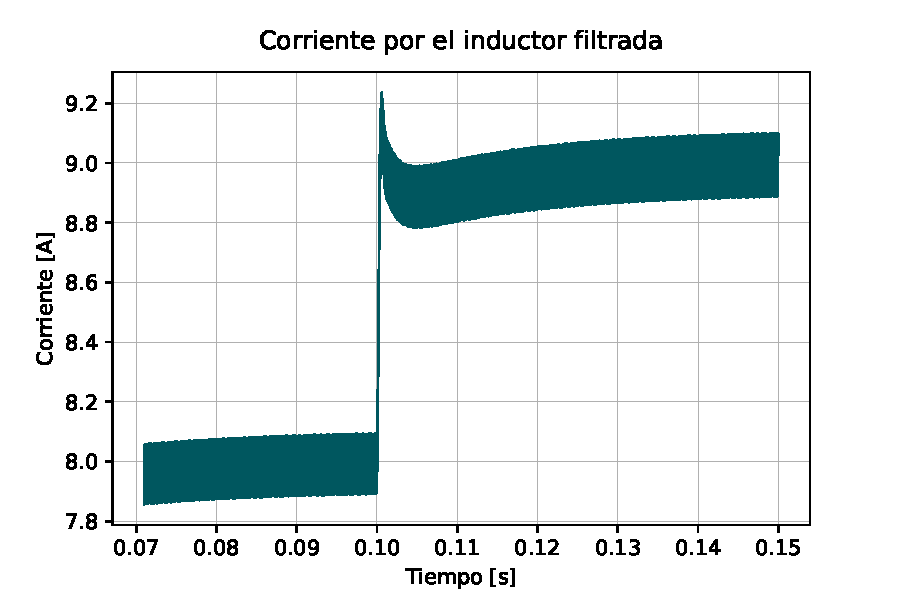
\includegraphics[width=0.45\textwidth]{Imágenes/Diseño del control/Simulación del lazo de corriente/Corriente por el inductor filtrada.pdf}}
  \hspace{3.5mm}
  \subfloat[Tensión en la salida.]{\includegraphics[width=0.45\textwidth]{Imágenes/Diseño del control/Simulación del lazo de corriente/Tensión en la salida.pdf}}
  \caption{Formas de onda obtenidas en la simulación del lazo de control de corriente.}
  \label{formas-onda-lazo-corriente}
\end{figure}

\begin{figure}[hbt!]
  \centering
  \subfloat[Corriente por el inductor en detalle.]{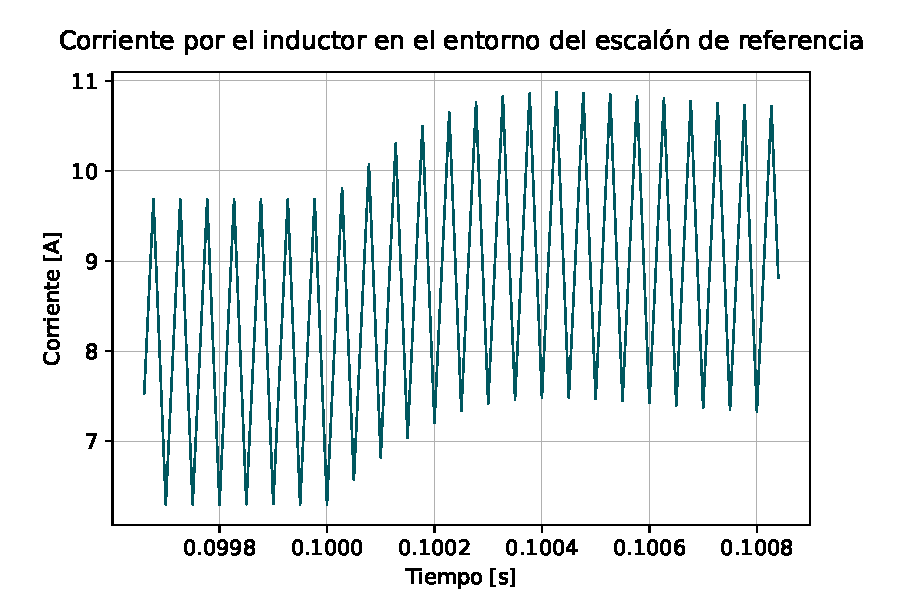
\includegraphics[width=0.45\textwidth]{Imágenes/Diseño del control/Simulación del lazo de corriente/Corriente por el inductor en entorno.pdf}}    
  \hspace{3.5mm}
  \subfloat[Corriente por el inductor filtrada en detalle.]{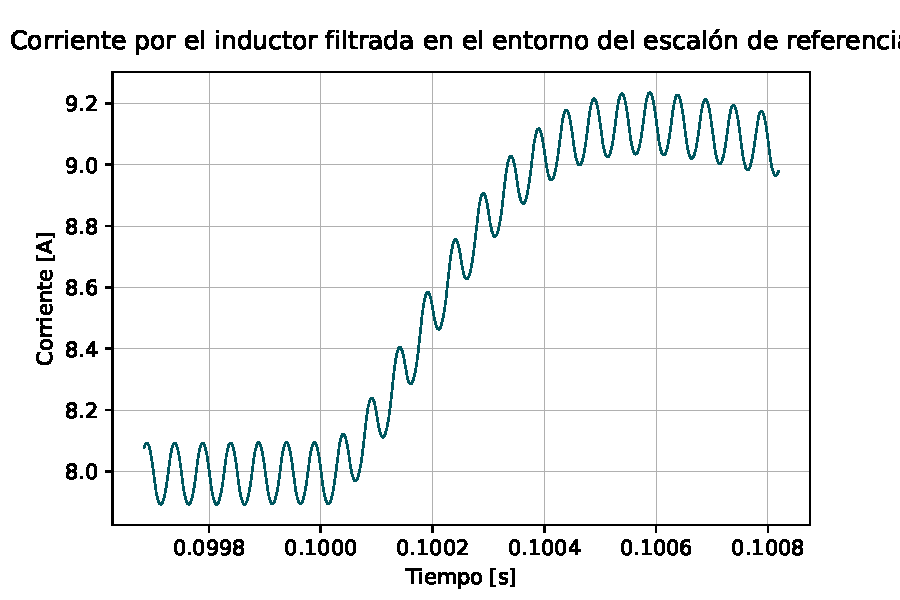
\includegraphics[width=0.45\textwidth]{Imágenes/Diseño del control/Simulación del lazo de corriente/Corriente por el inductor filtrada en entorno.pdf}}
  \hspace{3.5mm}
  \caption{Corriente del inductor alrededor del entorno del escalón unitario de corriente.}
  \label{formas-onda-filtradas-lazo-corriente}
\end{figure}

\subsection{Diseño del lazo externo de tensión}

Para el diseño del lazo de control de tensión y poder controlar la tensión de salida del convertidor, se implementa la estrategia de control que se muestra en la Figura \ref{lazo-tension}

\begin{figure}[hbt!]
  \centering
  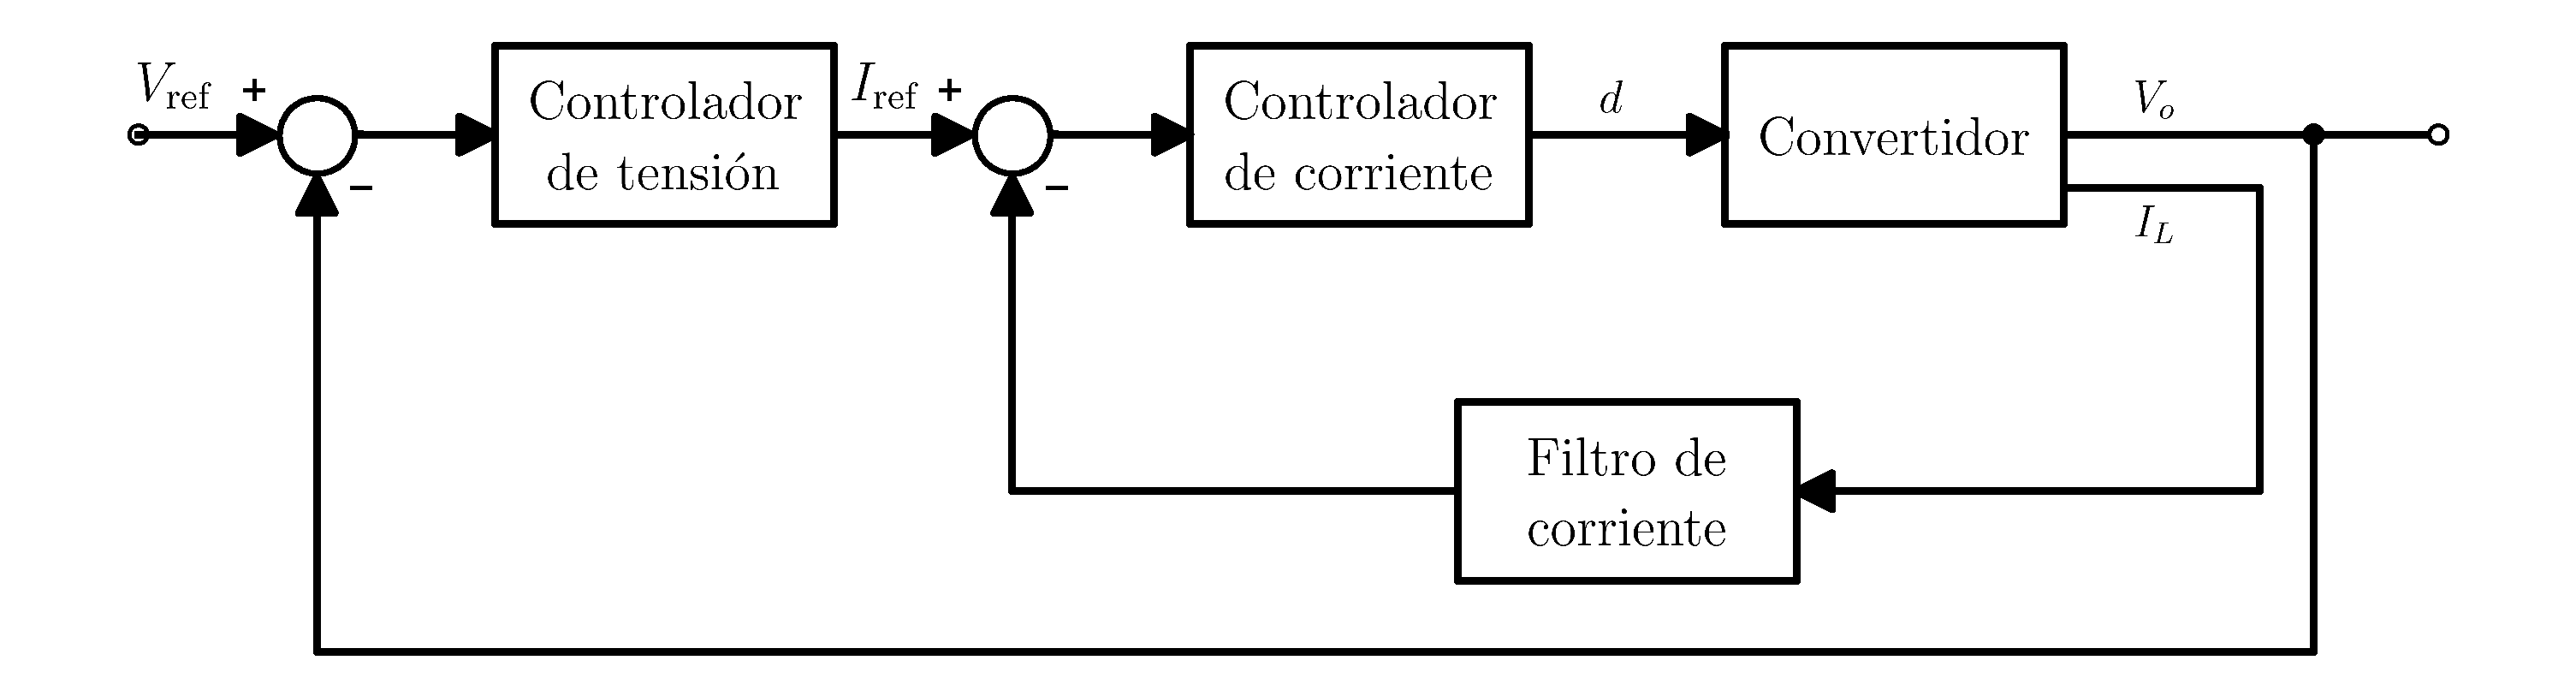
\includegraphics[width=0.80\columnwidth]{Imágenes/Diseño del control/Lazo de control de tensión.pdf}
  \caption{Ilustración del lazo de control de tensión.}
  \label{lazo-tension}
\end{figure} 

Como se puede observar, el lazo de corriente queda anidado dentro del de tensión y es visto como parte de la planta a controlar por este. Por lo tanto, es necesario realizar una expansión del modelo del sistema que incluya al lazo de control de corriente. Este debe incluir al convertidor, al lazo interno de corriente, y a su filtro correspondiente. Desarrollando mediante modelos de estados al controlador PI de corriente y a su filtro se obtienen las ecuaciones en diferencias correspondientes:

\begin{equation*}
  \begin{split}
    & x_1\left[n+1\right] = I_{\mathrm{ref}} - x_2\left[n\right]
    \\
    & x_2\left[n+1\right] = 0.0150796 \, i_L\left[n\right] + 0.98492 \, x_2\left[n\right]
  \end{split}
  \label{ecuaciones-extra}
\end{equation*}

Reemplazando,

\begin{equation*}
  d\left[n\right] = \left( I_{\mathrm{ref}} - x_2\left[n\right] \right) \, K_p + K_i \, T_s \, x_1\left[n\right]
\end{equation*}

Y sustituyendo con los valores correspondientes al controlador PI de corriente:

\begin{equation*}
  d\left[n\right] = 0.02 \, I_{\mathrm{ref}} -  0.02\, x_2\left[n\right] + 17.04 \times 10^{-6} \, x_1\left[n\right]
  \label{ecuacion-extra}
\end{equation*}

Expresando las ecuaciones diferenciales del modelo linealizado del convertidor dados por las \mbox{Ecuaciones \ref{sistema-modelo-lineal}} en ecuaciones en diferencias considerando un tiempo de muestro de \SI{1.42}{\micro\second} y el punto de trabajo establecido anteriormente, se obtiene:

\begin{equation*}
  \begin{split}
    &i_L \left[n+1\right] = i_L\left[n\right] - 0.00355 \, v_o\left[n\right] + 0.355 \, d\left[n\right]
    \\
    & v_o\left[n+1\right] = 0.00323 i_L\left[n\right] + 0.99996 \, v_o\left[n\right] - 0.00430 d \left[n\right]
  \end{split}
  \label{ecuaciones-originales-expansion}
\end{equation*}

Luego, expandiendo el sistema con las Ecuaciones \ref{ecuaciones-extra}, \ref{ecuacion-extra} y \ref{ecuaciones-originales-expansion}:

\begin{equation*}
  \begin{split}
    &i_L \left[n+1\right] = i_L\left[n\right] - 0.00355 \, v_o\left[n\right] + 0.355 \, \left[ 0.02 \, I_{\mathrm{ref}} -  0.02\, x_2\left[n\right] + 17.04 \times 10^{-6} \, x_1\left[n\right] \right]
    \\
    & v_o\left[n+1\right] = 0.00323 i_L\left[n\right] + 0.99996 \, v_o\left[n\right] - 0.00430 \left[ 0.02 \, I_{\mathrm{ref}} -  0.02\, x_2\left[n\right] + 17.04 \times 10^{-6} \, x_1\left[n\right] \right]
    \\
    & x_1\left[n+1\right] = I_{\mathrm{ref}} - x_2\left[n\right]
    \\
    & x_2\left[n+1\right] = 0.0150796 \, i_L\left[n\right] + 0.98492 \, x_2\left[n\right]
  \end{split}
\end{equation*}

Distribuyendo términos y generando una representación matricial:

\begin{align*}
  \boxed{
  \begin{bmatrix}
    i_L\left[n+1\right]\\
    v_o\left[n+1\right]\\  
    x_1\left[n+1\right]\\  
    x_2\left[n+1\right]\\  
  \end{bmatrix}
  =
  \begin{bmatrix}
    1 & -0.00355 & 6.0492 \times 10^{-6} & -7.1 \times 10^{-3}\\
    0.99996 & 3.23 \times 10^{-3} & -73.272 \times 10^{-9} & 86 \times 10^{-6}\\
    0 & 0 & 0 & -1 \\
    15.0796 \times 10^{-3} & 0 & 0 & 0.98492 \\
  \end{bmatrix}
  \,
  \begin{bmatrix}
    i_L\left[n\right]\\
    v_o\left[n\right]\\  
    x_1\left[n\right]\\  
    x_2\left[n\right]\\  
  \end{bmatrix}
  +
  \begin{bmatrix}
    7.1 \times 10^{-3}\\
    86 \times 10^{-6}\\  
    1\\  
    0\\  
  \end{bmatrix}
  \,
  I_{\mathrm{ref}}
  }
\end{align*}

Este sistema discreto expandido representa a la planta a lazo cerrado de corriente. Una cuestión crítica a tener en cuenta a la hora de empezar a diseñar el lazo de tensión es que su dinámica debe ser aproximadamente un orden de magnitud más lenta que la del lazo de corriente, para que esta pueda seguir su referencia de forma adecuada y sin provocar un comportamiento oscilatorio.

La sintonía del controlador de tensión fue realizada con el mismo método que el utilizado para sintonizar el PI de corriente, mediante una aproximación lineal y ajustes progresivos basados en la respuesta temporal observada. El siguiente controlador proporcional-integral de tensión fue obtenido:

\begin{equation*}
  \mathrm{PI}_U = K_{p_U} + \frac{K_{i_U} \, T_s}{z-1} 
\end{equation*}

\begin{equation*}
  \boxed{\mathrm{PI}_U = 0.2 + \frac{15 \cdot \, 1.6 \times 10^{-6}}{z-1}}
\end{equation*}

Lo que implica $K_{p_U} = 0.2$ y $K_{i_U} = 15$. En la Figura \ref{simulacion-modelo-real-tension} se ilustra el diagrama en bloques armado para la simulación del modelo real. En el lazo de control se puede observar el control de la tensión junto con el control de corriente anidado, y el muestreo de las variables de estado del convertidor electrónico. 

\begin{figure}[hbt!]
  \centering
  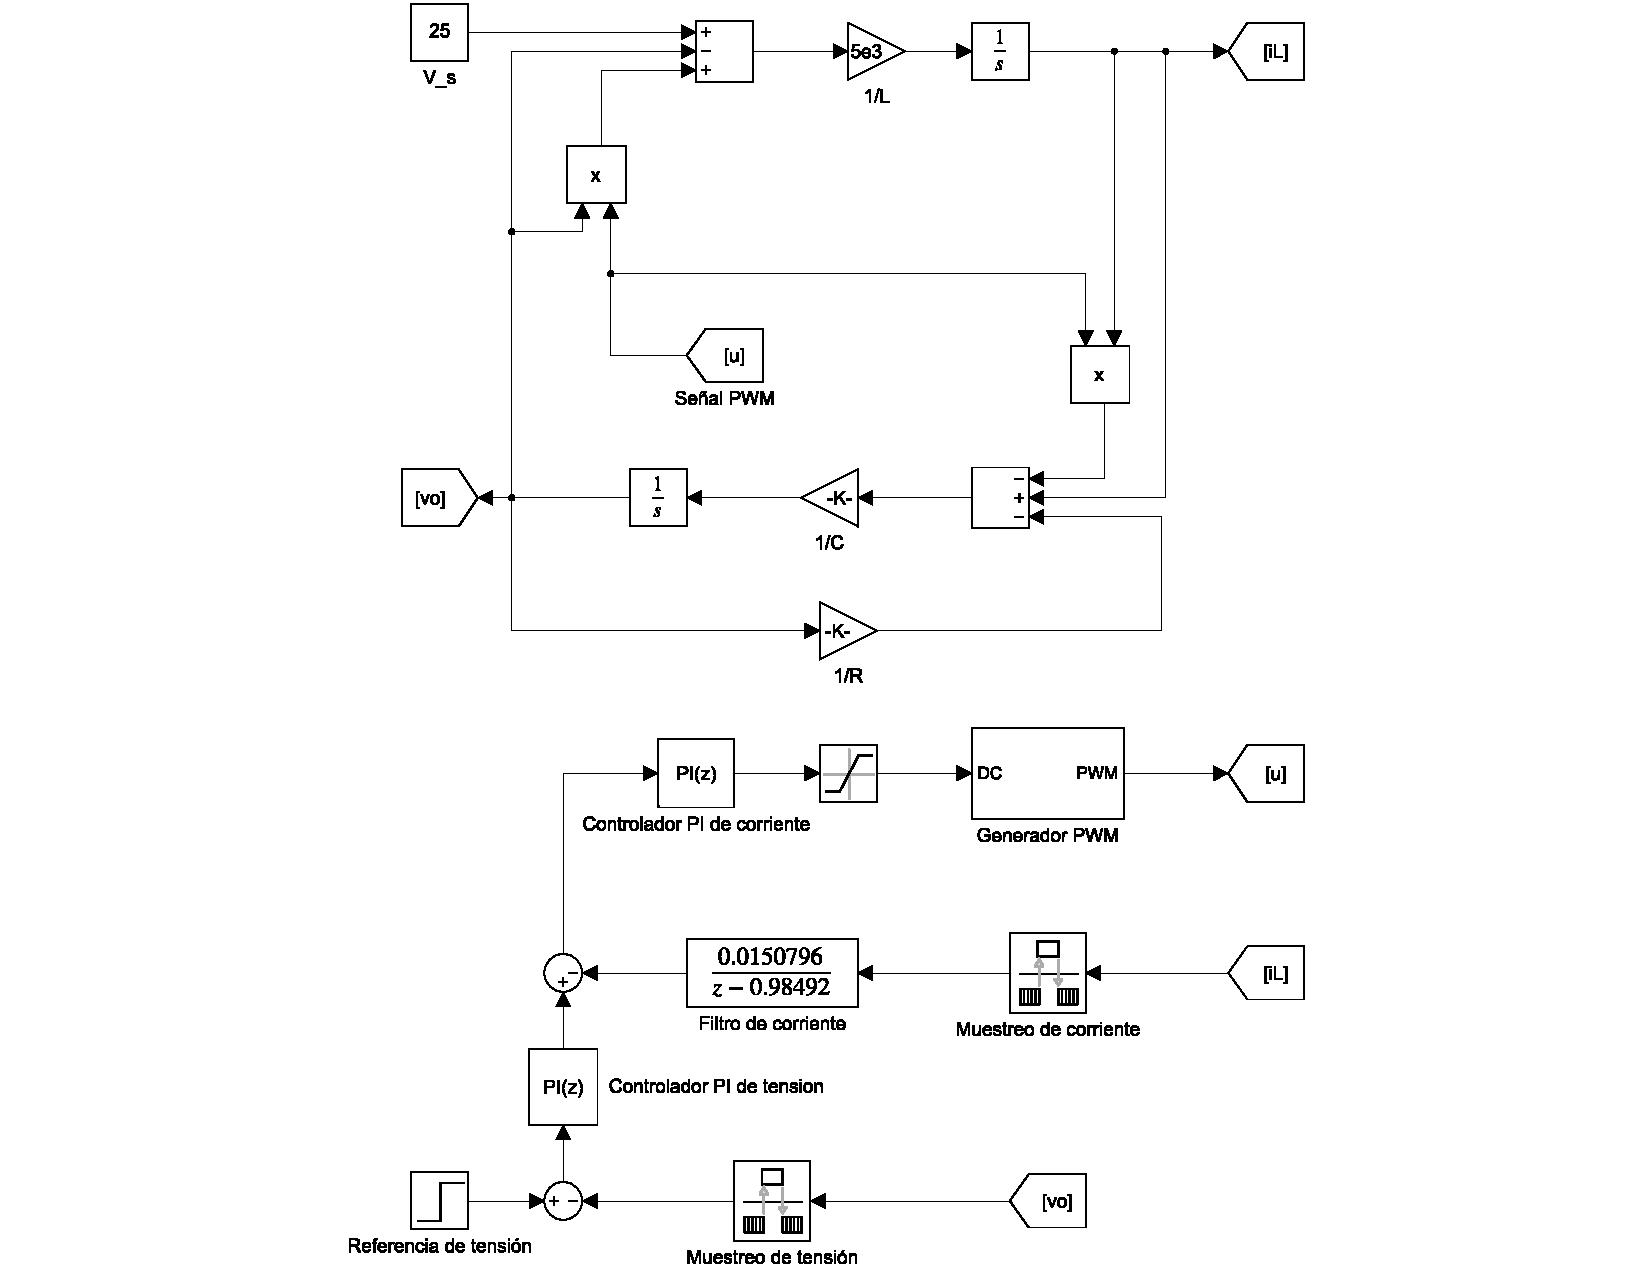
\includegraphics[width=0.75\columnwidth]{Imágenes/Diseño del control/Simulación del lazo de tensión/Simulación real del lazo de tensión.pdf}
  \caption{Simulación real del lazo de control de tensión.}
  \label{simulacion-modelo-real-tension}
\end{figure} 

La simulación realizada para este sistema es similar a la del lazo de corriente. Se inyectó nuevamente un escalón a la referencia de tensión que varía de \SI{50}{\volt} a \SI{55}{\volt} a los \SI{0.25}{\second}, y se observan las mismas formas de onda graficadas anteriormente. En el escalón de referencia no se discierne un sobrepico de tensión en la salida, y nuevamente utilizando las herramientas de Simulink\textsuperscript\textregistered \hspace{0.6pt} se mide el tiempo de establecimiento al 2\%, el cual resulta ser de aproximadamente \SI{70}{\milli\second}.

\begin{figure}[hbt!]
  \centering
  \subfloat[Referencia de tensión.]{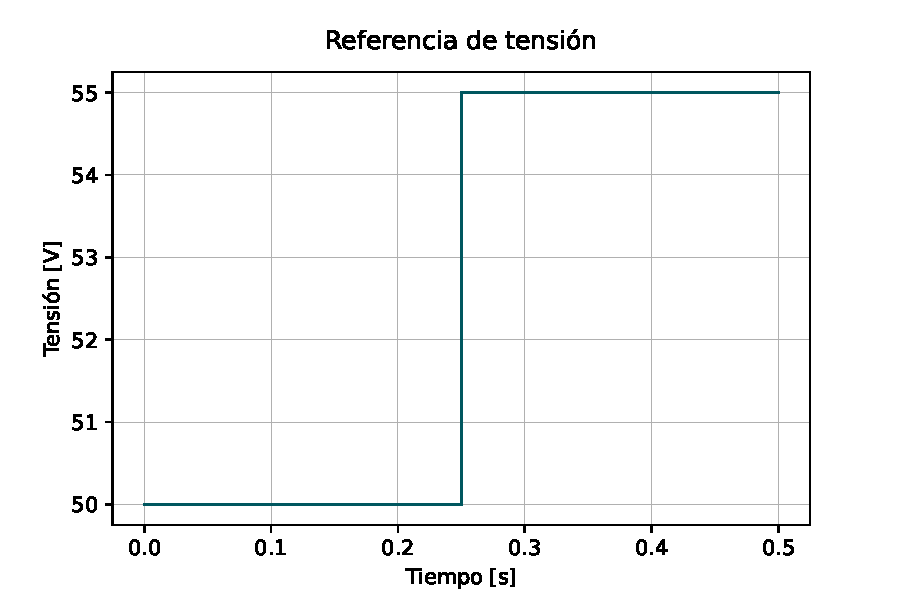
\includegraphics[width=0.45\textwidth]{Imágenes/Diseño del control/Simulación del lazo de tensión/Referencia de tensión.pdf}}    
  \hspace{3.5mm}
  \subfloat[Tensión en la salida.]{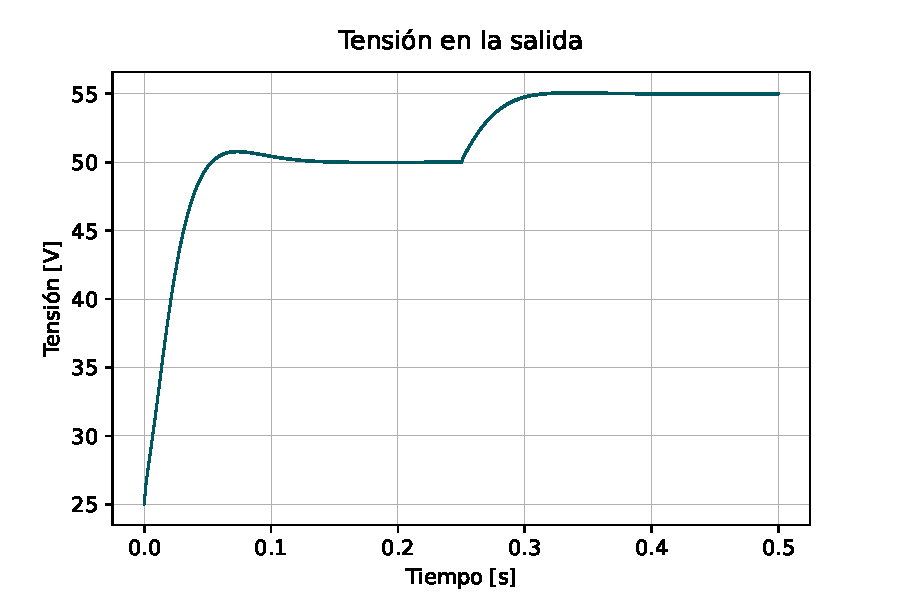
\includegraphics[width=0.45\textwidth]{Imágenes/Diseño del control/Simulación del lazo de tensión/Tensión en la salida.pdf}}
  \hspace{3.5mm}
  \subfloat[Corriente por el inductor filtrada.]{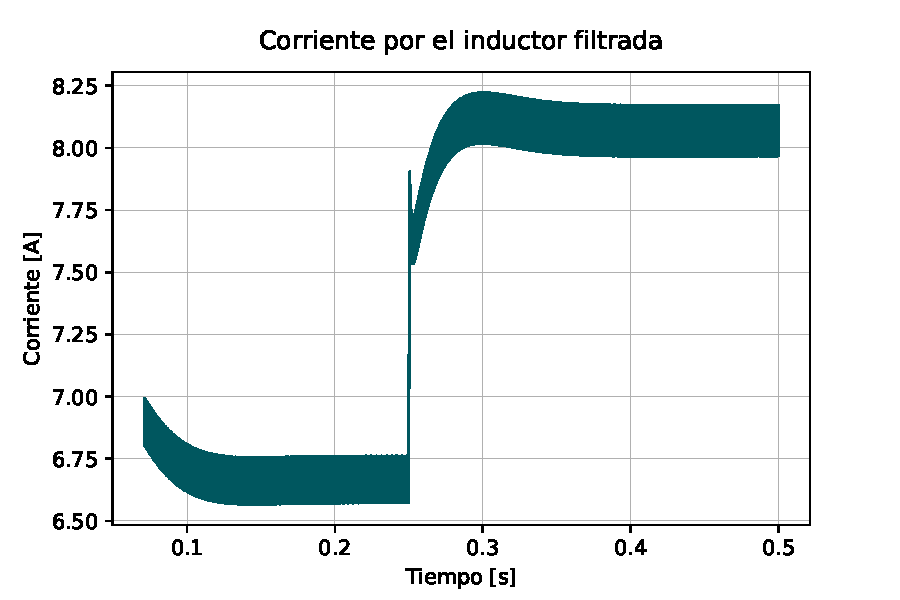
\includegraphics[width=0.45\textwidth]{Imágenes/Diseño del control/Simulación del lazo de tensión/Corriente por el inductor filtrada.pdf}}
  \hspace{3.5mm}
  \subfloat[Corriente por el inductor.]{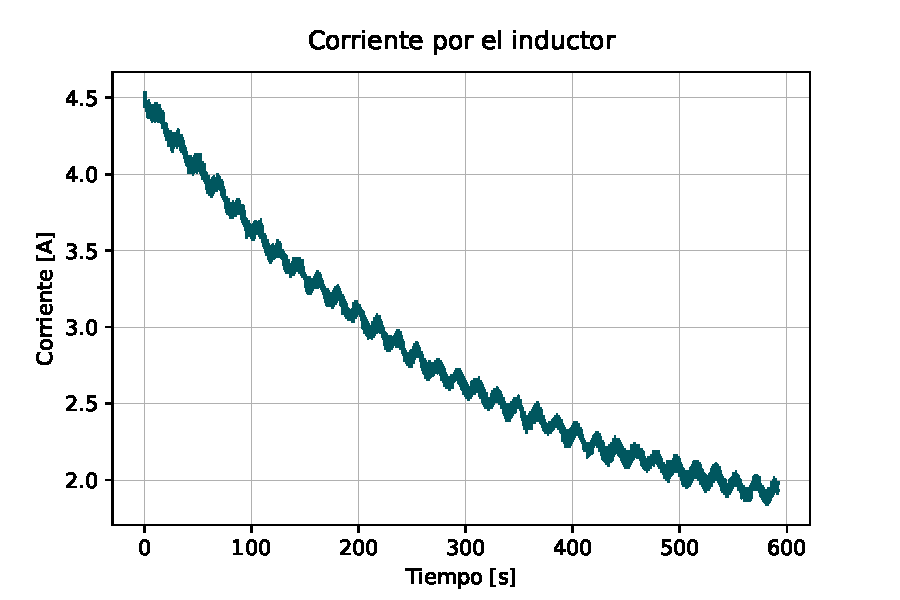
\includegraphics[width=0.45\textwidth]{Imágenes/Diseño del control/Simulación del lazo de tensión/Corriente por el inductor.pdf}}
  \caption{Formas de onda obtenidas en la simulación del lazo de control de tensión.}
  \label{formas-onda-lazo-tension}
\end{figure}

\subsubsection{Variación de la resistencia de carga}

La última prueba en Simulink\textsuperscript\textregistered \hspace{0.6pt} se realiza modificando la carga conectada al convertidor elevador a lazo cerrado de tensión. Esta simulación se aproxima mejor a una situación real en la cual la demanda de la carga presenta una variación mientras está conectada al sistema.

Esta simulación consiste en hacer variar la resistencia de carga de un valor incial de \SI{15}{\ohm} a un valor de \SI{12}{\ohm} en t = \SI{0.25}{\second}. En la Figura \ref{var-carga-simulink} puede observarse la modificación realizada al modelo para poder realizar esta prueba.

\begin{figure}[hbt!]
  \centering
  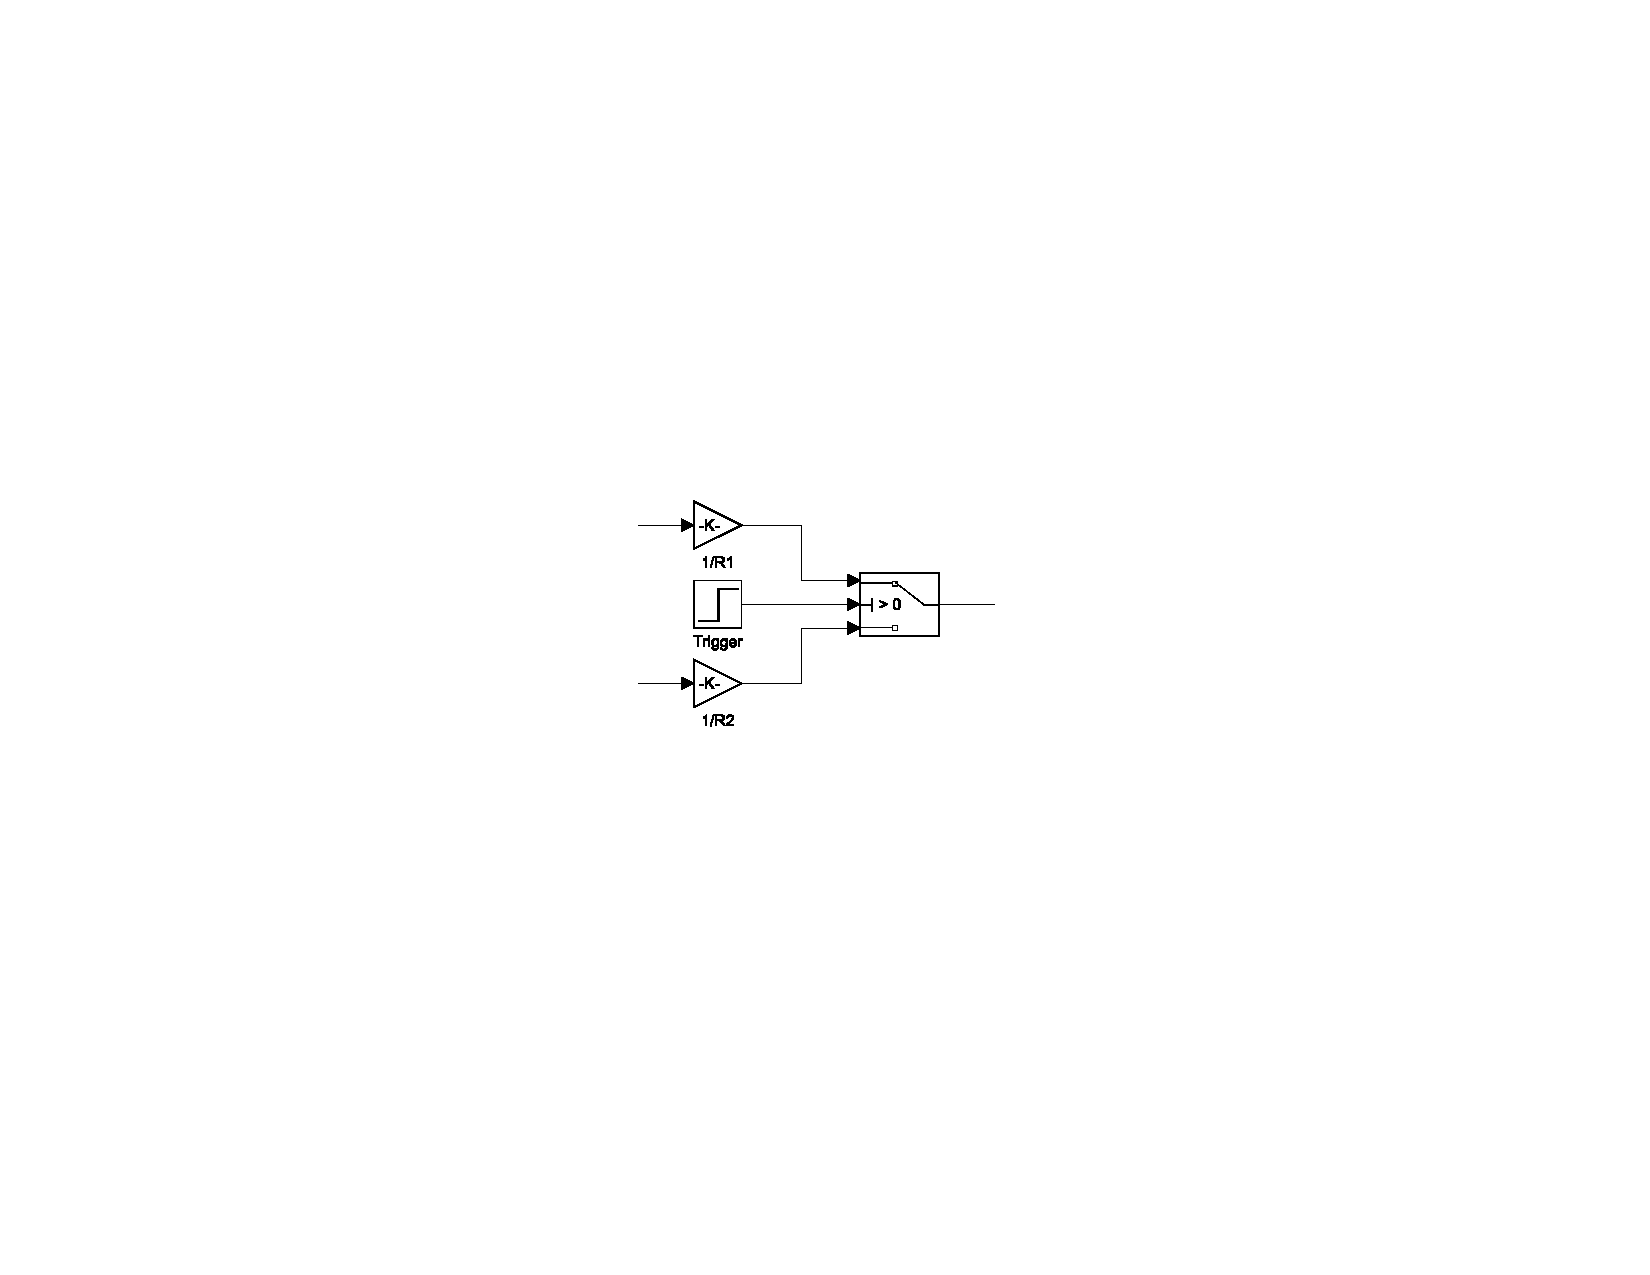
\includegraphics[width=0.35\columnwidth]{Imágenes/Diseño del control/Variación de parámetros de carga/Variación de resistencia de carga/Estructura en Simulink.pdf}
  \caption{Bloques reemplazados para simular una variación de carga.}
  \label{var-carga-simulink}
\end{figure} 

Simulando por un tiempo de \SI{0.5}{\second} a la variación de la resistencia de carga, la tensión que cae en ella, la corriente de por el inductor filtrada, y la acción de control, se obtienen la Figura \ref{formas-onda-var-carga}. Aquí se puede observar la adecuada respuesta del sistema de control ante este tipo de perturbaciones sin presentar sobrepicos y con un comportamiento suave y lo suficientemente rápido para volver a la tensión establecida a partir de la referencia elegida.

\begin{figure}[hbt!]
  \centering
  \subfloat[Variación de la resistencia.]{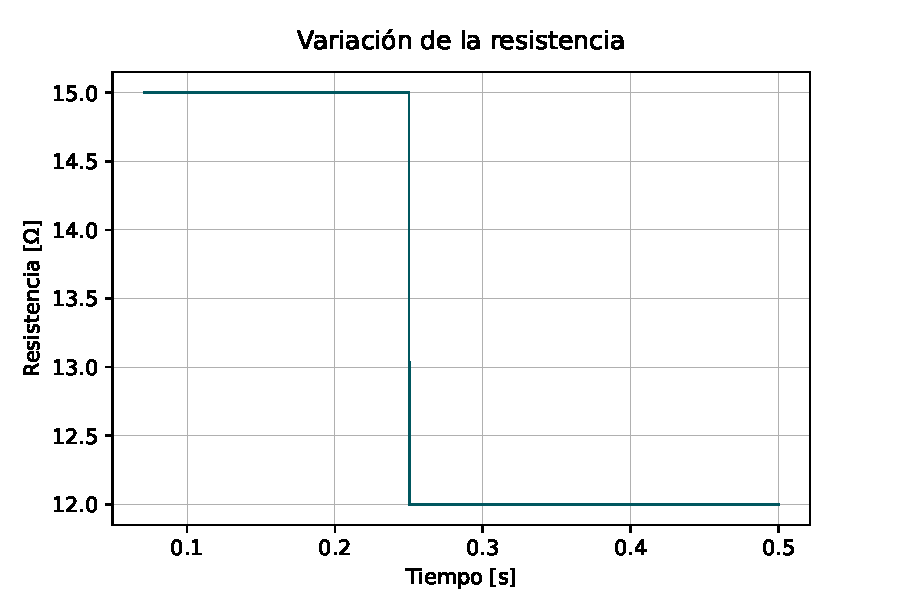
\includegraphics[width=0.45\textwidth]{Imágenes/Diseño del control/Variación de parámetros de carga/Variación de resistencia de carga/Variación de la resistencia.pdf}}    
  \hspace{3.5mm}
  \subfloat[Tensión en la salida.]{\includegraphics[width=0.45\textwidth]{Imágenes/Diseño del control/Variación de parámetros de carga/Variación de resistencia de carga/Tensión en la salida.pdf}}
  \hspace{3.5mm}
  \subfloat[Corriente por el inductor filtrada.]{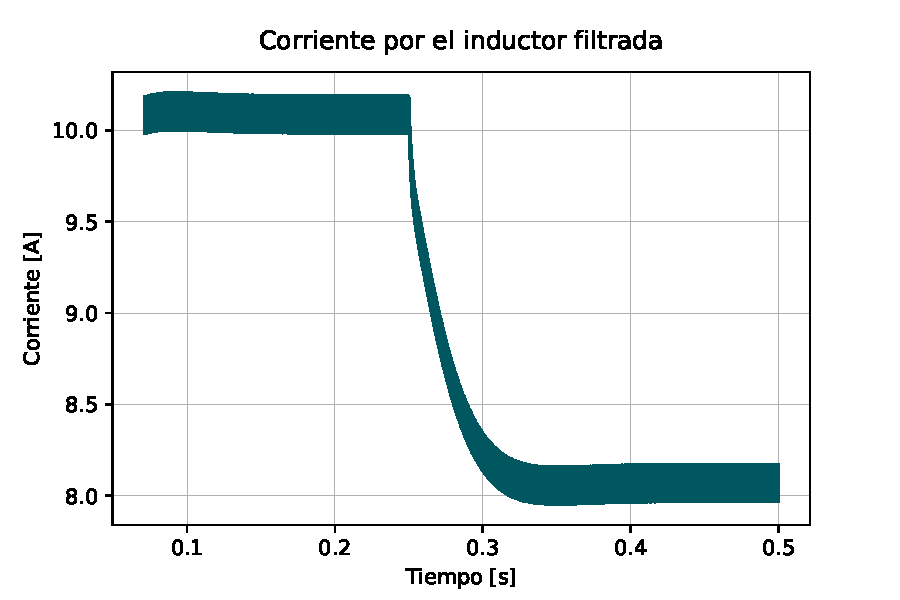
\includegraphics[width=0.45\textwidth]{Imágenes/Diseño del control/Variación de parámetros de carga/Variación de resistencia de carga/Corriente por el inductor filtrada.pdf}}
  \hspace{3.5mm}
  \subfloat[Acción de control.]{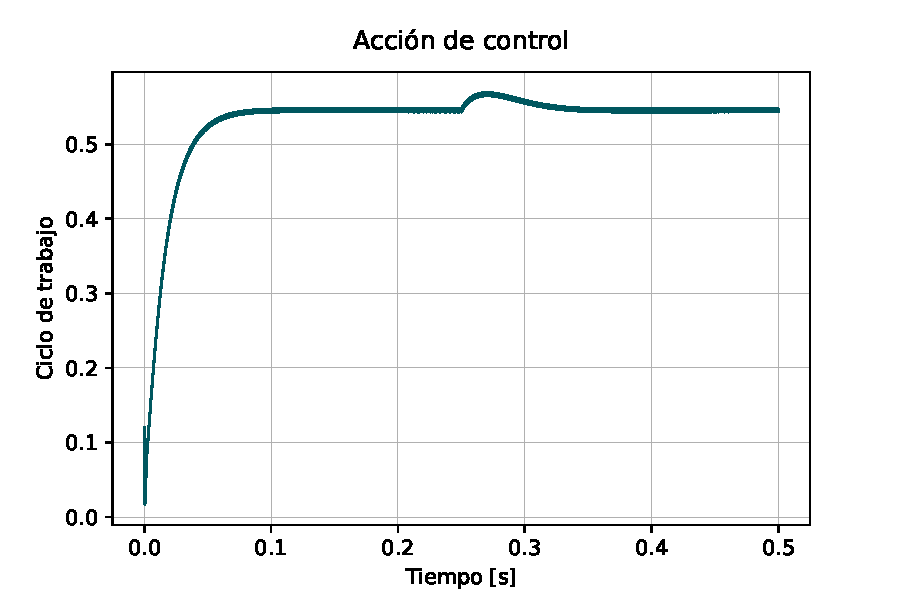
\includegraphics[width=0.45\textwidth]{Imágenes/Diseño del control/Variación de parámetros de carga/Variación de resistencia de carga/Acción de control.pdf}}
  \caption{Formas de onda obtenidas en la simulación de una variación de la resistencia de carga.}
  \label{formas-onda-var-carga}
\end{figure}

\section{Resumen}

En este capítulo se ha expuesto el proceso de diseño del sistema de control a implementar, a través del desarrollo de las ecuaciones matemáticas que rigen a sus componentes (el filtro y los controladores), así como las que describen a un modelo del sistema lo suficientemente sencillo para poder utilizar las herramientas convencionales de análisis. 

Además se incluyeron simulaciones en cada etapa del proceso para corroborar el correcto funcionamiento de la acción de control provista por el sistema diseñado, y por último se realizaron una serie de simulaciones con el propósito de emular eventos que puedan ocurrir en el sistema real, para observar el comportamiento satisfactorio del sistema en el lazo cerrado de control creado.

En el próximo capítulo se muestra la programación de este sistema en el circuito de desarrollo utilizado para este trabajo, una FPGA con el lenguaje VHDL, y se realizan nuevas simulaciones en el entorno de este lenguaje HDL para confirmar su correcta implementación. 

\newpage